%%
%% Arquivo principal adaptado para:
%% - Trabalho de Conclusão de Curso de Graduação - Eng. Computação e Mecatrônica - UFRN
%%
%% NOTA: A PUBLICAÇÃO DESTE MODELO VISA APENAS ORIENTAR OS PÓS-GRADUANDOS
%% NA PREPARAÇÃO DE SEUS TEXTOS. O PPgEE DA UFRN NÃO PROVÊ ASSISTÊNCIA NO
%% USO DAS FERRAMENTAS NECESSÁRIAS AO USO DESTE MODELO (LATEX, XFIG, ETC.)
%%
%% Baseado no modelo prévio para Tese de Pós Graduação PPGEEC do Prof. Dr.Adelardo Medeiros, dezembro de 2005.
%% Revisado pelos alunos de Metodologia da Pesquisa Científica de 2016.1.


%% -------------------------------------------------------------------------
%%
%% NOTA: Modelo adaptado em Julho de 2022 para template de TCC em Eng. de Computação 
%% e Mecatrônica da UFRN/CT.
%%
%% Válber César Cavalcanti Roza (Sec. de Coordenação de Eng.Mecatrônica CTEC/UFRN),20 de Julho, 2022.
%% Revisado pelo secretariado das Coordenações dos respectivos cursos.
%%
%% -------------------------------------------------------------------------


% DEFINIÇÕES GLOBAIS

% Esta primeira linha dá informações gerais sobre o documento.
% PARA A VERSÃO FINAL:
% papel A4, letra grande (12pt), openright (capítulos só iniciam em
% página direita, se necessário incluindo uma página em branco),
% twoside (o documento vai ser impresso em frente e costa)
\documentclass[a4paper,12pt,openright,twoside]{book}
% PARA A QUALIFICAÇÃO E PARA A VERSÃO INICIAL:
% papel A4, letra grande (12pt), openany (capítulos iniciam em
% qualquer página), oneside (o documento vai ser impresso só na frente)
%\documentclass[a4paper,12pt,openany,oneside]{book}


% Use estes pacotes para poder digitar diretamente as letras com acento
% e para que a hifenização funcione corretamente
\usepackage[utf8]{inputenc}
\usepackage{ae}
% Para usar fontes standard ao invés das do LaTeX (gera melhores PDFs)
\usepackage{pslatex}
% Para a hifenização em português
\usepackage[portuges, brazil]{babel}
% Para que os primeiros parágrafos das seções também sejam indentados
\usepackage{indentfirst}
% Para poder incluir gráficos (figuras)
\usepackage{graphicx}
% Para poder fazer glossário ou lista de símbolos
% Use a segunda opção se quiser incluir na definição do símbolo a
% página e/ou a equação onde ela foi definida
\usepackage[portuguese,noprefix]{nomencl}
%\usepackage[portuguese,noprefix,refeq,refpage]{nomencl}
% Para permitir espaçamento simples, 1 1/2 e duplo
\usepackage{setspace}
% Para usar alguns comandos matemáticos avançados muito úteis
\usepackage{amsmath}
\usepackage{amsfonts}
% Para poder usar o ambiente "comment"
\usepackage{verbatim}
% Para poder ter tabelas com colunas de largura auto-ajustável
\usepackage{tabularx}
% Para executar um comando depois do fim da página corrente
\usepackage{afterpage}
% Para formatar URLs (endereços da Web)
\usepackage{url}
% Para reduzir os espaços entre os ítens (itemize, enumerate, etc.)
% Este pacote não faz parte da distribuição padrão do LaTeX.
\usepackage{lib/noitemsep}
% Para as citações bibliográficas
%\usepackage[alf]{abntex2cite}
\usepackage[abbr]{lib/harvard}	% As chamadas são sempre abreviadas
%\harvardparenthesis{square}	% Colchetes nas chamadas
%\harvardyearparenthesis{round}	% Parêntesis nos anos das referências
%\renewcommand{\harvardand}{e}	% Substituir "&" por "e" nas referências

% PACOTES OPCIONAIS
% Para posicionar uma figura onde quiser
\usepackage{float}
% Para poder incluir arquivos Postscript com cores (do Xfig, por exemplo)
\usepackage{color}
% Para ter células em tabelas que ocupam mais de uma linha
\usepackage{multirow}
% Para poder ter tabelas longas em mais de uma página
%\usepackage{longtable}
% Para poder escrever partes do texto em "n" colunas
%\usepackage{multicol}
% Se você quiser personalizar os cabeçalhos das páginas
%\usepackage{fancyheadings}
% Para incluir algoritmos e listagens de códigos
%\usepackage{listings}
% Para incluir pseudocódigos
\usepackage[portuguese, ruled, linesnumbered]{algorithm2e}
% Capítulos com títulos em um formato "decorado"
\usepackage{lib/capitulos}
% Hiperreferências dentro do texto e montagem dos links do índices dos
% para os leitores de pdf (deve ser o último pacote a ser inserido).
\usepackage[breaklinks]{hyperref}
% Referência correta de ambientes flutuantes (como figuras, tabelas e algoritmos).
\usepackage[all]{hypcap}

\hypersetup{
    colorlinks=true,
    linkcolor=black,
    filecolor=magenta,      
    urlcolor=cyan,
    pdftitle={Sistema de controle para Andador inteligente},
    % pdfpagemode=FullScreen,
}

% NOVOS COMANDOS

% As definições dos novos comandos estão agrupadas no arquivo "comandos.tex"
% Esta separação é opcional: se você preferir, pode por as definições
% diretamente neste arquivo
% newcommand define novos comandos, que podem passar a ser usados da
% mesma forma que os comandos LaTeX de base.

% Implicação em fórmulas
\newcommand{\implica}{\quad\Rightarrow\quad} %Meio de linha
\newcommand{\implicafim}{\quad\Rightarrow}   %Fim de linha
\newcommand{\tende}{\rightarrow}
\newcommand{\BibTeX}{\textsc{B\hspace{-0.1em}i\hspace{-0.1em}b\hspace{-0.3em}}\TeX}

% Fração com parentesis
\newcommand{\pfrac}[2]{\left(\frac{#1}{#2}\right)}

% Transformada de Laplace e transformada Z
%\newcommand{\lapl}{\makebox[0cm][l]{\hspace{0.1em}\raisebox{0.25ex}{-}}\mathcal{L}}
\newcommand{\lapl}{\pounds}
\newcommand{\transfz}{\mathcal{Z}}

% Não aparecer o número na primeira página dos capítulos
\newcommand{\mychapter}[1]{\chapter{#1}\thispagestyle{empty}}

% Os capítulos sem número
\newcommand{\mychapterast}[1]{\chapter*{#1}\thispagestyle{empty}
\chaptermark{#1}
\afterpage{\markboth{\uppercase{#1}}{\rightmark}}
\markboth{\uppercase{#1}}{}
}

% Seções sem número
\newcommand{\mysectionast}[1]{\section*{#1}
\addcontentsline{toc}{section}{#1}
\markright{\uppercase{#1}}
}

% No tabularx, as celulas devem ser centradas verticalmente
\renewcommand{\tabularxcolumn}[1]{m{#1}}

% Células centralizadas horizontalmente no tabularx
\newcolumntype{C}{>{\centering\arraybackslash}X}

%% Abrevia figuras e tabelas
%\def\figurename{Fig.}
%\def\tablename{Tab.}


%
% As margens
%

% Direção horizontal

% Margem interna
% Nas páginas ímpares
\setlength{\oddsidemargin}{3.5cm}         % Margem real desejada
% Nas páginas pares
\setlength{\evensidemargin}{2.5cm}        % Margem real desejada
% Largura do texto
\setlength{\textwidth}{15cm}
% As margens laterais no LaTeX são sempre 1 polegada maiores do que as
% fixadas. Se foi fixada \setlength{\oddsidemargin}{3.5cm}, a margem
% real seria de 3.5+2.54=6.04cm. Para permitir que você não tenha que
% fazer esta conta, pode usar o número desejado nas linhas anteriores
% e a gente subtrai 1in nas próximas linhas
\addtolength{\oddsidemargin}{-1in}
\addtolength{\evensidemargin}{-1in}
% Note que a margem direita não é fixada diretamente:
% ela é obtida subtraindo-se os outros valores da largura da página.
% 3.5+15+x=21cm (largura A4) -> x = margem externa = 2.5cm

% Direção vertical

% Margem superior (entre o topo da folha e o cabeçalho), altura do
% cabeçalho e distância entre o fim do cabeçalho e o início do texto
\setlength{\topmargin}{2.0cm}             % Margem real desejada
\setlength{\headheight}{1.0cm}
\setlength{\headsep}{1.0cm}
% Altura do texto (sem cabeçalho e rodapé)
\setlength{\textheight}{22.7cm}
% Distância do fim do texto ao rodapé
\setlength{\footskip}{1.0cm}
% A margem superior no LaTeX é sempre 1 polegada maior do que a
% fixada. Se foi fixada \setlength{\topmargin}{2.0cm}, a margem
%real seria de 2.0+2.54=4.54cm. Para permitir que você não tenha que
% fazer esta conta, pode usar o número desejado na linha anterior
% e a gente subtrai 1in na próxima linha
\addtolength{\topmargin}{-1in}
% Note que a margem inferior não é fixada diretamente:
% ela é obtida subtraindo-se os outros valores, sem incluir o
% "footskip", da altura da página.
% 2.0+1.0+1.0+22.7+x=29.7cm (altura A4) -> x = margem inferior = 3cm

%
% O estilo das referências bibliográficas
%

\bibliographystyle{bibliografia/ppgee}

%
% O espaçamento entre linhas
%

% As páginas iniciais são sempre em espaçamento simples
\singlespacing

% Para a criação do glossário (ou lista de símbolos)
\makenomenclature

% Lista de arquivos a serem processados. Estes comandos "includeonly" são
% dispensáveis e devem obrigatoriamente ser comentados na hora de gerar o
% documento definitivo. Eles servem para compilar apenas parte do documento.
% É útil, durante a redação, para que não se tenha de compilar todo o
% documento a cada vez que se faz uma alteração. Por exemplo, se eu estou
% fazendo alterações na dedicatória e as outras partes não têm interesse no
% momento, posso incluir (descomentar) a linha "\includeonly{preambulo}"
%\includeonly{rosto}
%\includeonly{catalograficos}
%\includeonly{preambulo}
%\includeonly{resumos}
%\includeonly{introducao/introducao}
%\includeonly{estilo/estilo}
%\includeonly{matematica/matematica}
%\includeonly{figuras/figuras}
%\includeonly{conclusao/conclusao}
%\includeonly{apendice/apendice}

% Inicia o texto
\begin{document}

% Paginas iniciais (sem numeração)
\pagestyle{empty}

% Página de rosto (capa interna)
%
% ********** Página de Rosto
%

% titlepage gera páginas sem numeração
\begin{titlepage}

\begin{center}

\small

\begin{tabularx}{\linewidth}{@{}l@{}C@{}r@{}}
\parbox[c]{3cm}{
\includegraphics[width=\linewidth]{./figuras/UFRN}} &
\begin{center}
\textsf{\textsc{Universidade Federal do Rio Grande do Norte\\
Centro de Tecnologia\\
Graduação em Engenharia de Computação}}
\end{center} &
\parbox[c]{3cm}{
\includegraphics[width=\linewidth]{./figuras/dca_logo.png}}
\end{tabularx}

\vfill
\LARGE
\textbf{Sistema de controle para Andador inteligente}
\vfill
\Large
\textbf{Samuel Cavalcanti}
\vfill

\normalsize

Orientador: Prof. Dr. Severino Lampeão
\\[2ex] Co-orientador: Prof. Dr. Zé Baiano % Opcional

\vfill

\hfill


\vfill

\large

Natal, RN, \today

\end{center}

\end{titlepage}

% Página de rosto (capa interna)
%
% ********** Página de Rosto
%

% titlepage gera páginas sem numeração
\begin{titlepage}

\begin{center}

\small

\begin{tabularx}{\linewidth}{@{}l@{}C@{}r@{}}
\parbox[c]{3cm}{
\includegraphics[width=\linewidth]{./figuras/UFRN}} &
\begin{center}
\textsf{\textsc{Universidade Federal do Rio Grande do Norte\\
Centro de Tecnologia\\
Graduação em Engenharia de Computação}}
\end{center} &
\parbox[c]{3cm}{
\includegraphics[width=\linewidth]{./figuras/dca_logo.png}}
\end{tabularx}

\vfill
\LARGE
\textbf{Sistema de controle para Andador inteligente}
\vfill
\Large
\textbf{Samuel Cavalcanti}
\vfill

\normalsize

Orientador: Prof. Dr. Severino Lampeão
\\[2ex] Co-orientador: Prof. Dr. Zé Baiano % Opcional

\vfill

\hfill
\parbox{0.5\linewidth}{\textbf{%
Trabalho de Conclusão de Curso de Graduação} na modalidade Monografia, 
submetido como parte dos requisitos necessários para 
conclusão do curso de Engenharia de Computação pela 
Universidade Federal do Rio Grande do Norte (UFRN/CT).
}

\vfill

\large

Natal, RN, \today

\end{center}

\end{titlepage}


% Ficha catalográfica: os dados catalográficos devem ser fornecidos
% pela BCZM.
% Só são incluídos na versão final da tese ou dissertação. Não são
% incluídos nem na proposta de tema de qualificação nem na versão
% preliminar da tese ou dissertação: nestes casos, comente a próxima linha.
%
% ********** Ficha Catalográfica
%

\newpage

\begin{center}

% Aqui não se usou \vfill porque o \vfill é construído internamente com
% o comando \vspace. Espaços verticais no início da folha com \vspace
% são ignorados. Para que isto não ocorra deve-se usar o \vspace*
% \vspace*{\fill} é como se fosse um \vfill*
\vspace*{\fill}

Divisão de Serviços Técnicos\\[1ex]
Catalogação da publicação na fonte.
UFRN / Biblioteca Central Zila Mamede

\vspace{2ex}

\begin{tabular}{|p{0.9\linewidth}|} \hline
\\ Cavalcanti, Samuel.\\
\hspace{1em} \tccTitle /
Samuel Cavalcanti - Natal, RN, \today \\
\hspace{1em} 19 p. \\
\\
\hspace{1em} Orientador: Pablo Javier Alsina \\
% \hspace{1em} Co-orientador: Zé Baiano \\
\\
\hspace{1em} Monografia - Universidade Federal do Rio Grande do Norte.
Centro de Tecnologia. Graduação em Engenharia de Computação. \\
\\
\hspace{1em} 1. Redação técnica - MOnografia. 2. \LaTeX - Monografia. 
I. Alsina, Pablo Javier.
\\
RN/UF/BCZM \hfill CDU XXX.YYY(YYY.0) \\ \hline
\end{tabular} 

\end{center}


% Assinaturas da banca, dedicatória e agradecimentos
% Só são incluídos na versão final da tese ou dissertação. Não são
% incluídos nem na proposta de tema de qualificação nem na versão
% preliminar da tese ou dissertação: nestes casos, comente a próxima linha.
%
% ********** Página de assinaturas
%

\begin{titlepage}

\begin{center}

\LARGE

\textbf{\tccTitle}

\vfill

\Large

\textbf{Samuel Cavalcanti}

\end{center}

\vfill

% O \noindent é para eliminar a tabulação inicial que normalmente é
% colocada na primeira frase dos parágrafos
\noindent
% Descomente a opção que se aplica ao seu caso
% Note que propostas de tema de qualificação nunca têm preâmbulo.
Monografia aprovada em \today, pela banca examinadora composta
pelos seguintes membros:

% Os nomes dos membros da banca examinadora devem ser listados
% na seguinte ordem: orientador, co-orientador (caso haja),
% examinadores externos, examinadores internos. Dentro de uma mesma
% categoria, por ordem alfabética

\begin{center}

\vspace{1.5cm}\rule{0.95\linewidth}{1pt}
\parbox{0.9\linewidth}{%
Prof. Dr. XXXXX (orientador) \dotfill\ DCA/UFRN}

\vspace{1.5cm}\rule{0.95\linewidth}{1pt}
\parbox{0.9\linewidth}{%
Prof. Dr. YYYYY (co-orientador) \dotfill\ MCA/UFRN}

\vspace{1.5cm}\rule{0.95\linewidth}{1pt}
\parbox{0.9\linewidth}{%
Prof. Dr. WWWWWW \dotfill\ DEM/UFFN}

\vspace{1.5cm}\rule{0.95\linewidth}{1pt}
\parbox{0.9\linewidth}{%
Profª Drª ZZZZZZ \dotfill\ DEE/UFRN}

\end{center}

\end{titlepage}

%
% ********** Dedicatória
%

% A dedicatória não é obrigatória. Se você tem alguém ou algo que teve
% uma importância fundamental ao longo do seu curso, pode dedicar a ele(a)
% este trabalho. Geralmente não se faz dedicatória a várias pessoas: para
% isso existe a seção de agradecimentos.
% Se não quiser dedicatória, basta excluir o texto entre
% \begin{titlepage} e \end{titlepage}

% \begin{titlepage}

% \vspace*{\fill}

% \hfill
% \begin{minipage}{0.5\linewidth}
% \begin{flushright}
% \large\it
% Aos meus ......
% \end{flushright}
% \end{minipage}

% \vspace*{\fill}

% \end{titlepage}

%
% ********** Agradecimentos
%

% Os agradecimentos não são obrigatórios. Se existem pessoas que lhe
% ajudaram ao longo do seu curso, pode incluir um agradecimento.
% Se não quiser agradecimentos, basta excluir o texto após \chapter*{...}

% \chapter*{Agradecimentos}
% \thispagestyle{empty}

% \begin{trivlist}  \itemsep 2ex

% \item Ao meu orientador e ao meu co-orientador, professores XXXXXX e YYYYYY, sou grato pela orientação.

% \item Ao secretário Halidaivson Stockhouse pela ajuda no andamento das coisas burocráticas do Curso.

% \item Aos colegas ....

% \item Aos demais colegas de graduação, pelas críticas e sugestões.

% \item À minha família pelo apoio durante esta jornada.

% \item À CAPES/CNPQ, pelo apoio financeiro.

% \item À Deus.

% \end{trivlist}


%
% O espaçamento entre linhas (ATENÇÃO A ESTA PARTE!)
%
%%%%%%%%%%%%%%%%%%%%%%%%%%%%%%%%%%%%%%%%%%%%%%%%%%%%%%%%%%%%%%%%%%%%%%%%%%%%
% PARA A VERSÃO FINAL:
% Deve ser usado espaçamento simples nas páginas de texto
\singlespacing
% PARA A QUALIFICAÇÃO E PARA A VERSÃO INICIAL:
% Deve ser usado espaçamento 1 1/2 nas páginas de texto
%\doublespacing
%%%%%%%%%%%%%%%%%%%%%%%%%%%%%%%%%%%%%%%%%%%%%%%%%%%%%%%%%%%%%%%%%%%%%%%%%%%%

% Resumo/Abstract
%
% ********** Resumo
%

% Usa-se \chapter*, e não \chapter, porque este "capítulo" não deve
% ser numerado.
% Na maioria das vezes, ao invés dos comandos LaTeX \chapter e \chapter*,
% deve-se usar as nossas versões definidas no arquivo comandos.tex,
% \mychapter e \mychapterast. Isto porque os comandos LaTeX têm um erro
% que faz com que eles sempre coloquem o número da página no rodapé na
% primeira página do capítulo, mesmo que o estilo que estejamos usando
% para numeração seja outro.
\mychapterast{Resumo}
O principal objetivo deste trabalho é criar um  sistema de
controle para o andador robótico inteligente que seja capaz de
posicionar o robô em uma posição em um ambiente livre de obstáculos,
também  este trabalho visa estudar e avaliar algoritmos de aprendizado
de máquina na elaboração do controlador. Primeiro foi feito um levantamento
literário sobre a utilização aprendizado de máquina para criação de
controladores cinemáticos em robôs moveis de acionamento diferencial,
segundo foi construído uma versão do robô no simulador Coppeliasim,
terceiro foi projetado um controlador cinemático, onde dois modelos
cinemáticos foram obtidos através da modelagem dos parâmetros de uma
rede neural artificial utilizando as equações que limitam o movimento
cinemático do robô, um modelo faz uma regressão não linear dos
parâmetros das equações, já outro modelo realiza uma regressão linear.
Os dados utilizados para o treinamento da rede são obtidos
através da criação de  algoritmos de coleta de dados e pré-processamento.
Já no controlador utiliza uma abordagem
clássica que possui  dois controladores
Proporcionais, integrais, derivativos (P.I.D),
onde ambos os parâmetros dos P.I.Ds foram obtidos empiricamente.
Para avaliar os modelos cinemáticos foi calculado o modelo analítico,
e coletado um conjunto de
dados de testes que foi utilizado para o cálculo do erro quadrático
médio para todos os modelos cinemáticos.
Para avaliar todo o sistema foi posicionado um alvo e observado o robô no 
seu trabalho em chegar até alvo mensurando a distância do robô até o
alvo e o seu angulo ao longo do tempo, o alvo foi posicionado em 4 lugares
diferentes. Os resultados do erro quadrático médio e os
gráficos de distância e angulo sobre o tempo 
mostraram que os dois modelos cinemáticos são equivalentes ao modelo
analítico. Comparando os parâmetros do modelo que realiza a
regressão não linear com o modelo analítico,
percebe-se os parâmetros como raio da roda e a distância entre as rodas,
se aproximaram da solução analítica, já para os ângulos das rodas foram
encontrados outros valores que quando somados se aproximam da solução
analítica. Foi concluído durante o levantamento literário que
utilizar a abordagem clássica é a melhor opção do que soluções com
aprendizado de máquina devido ao uso de memória e,
processamento com ambas soluções apresentando resultados equiparáveis.
Foi concluído que projetar o controlador cinemático encontrando o modelo
de forma analítica é mais simples do que usando algoritmos de aprendizado
de máquina, no entanto aplicar a modelagem  de sistemas para criar um
modelo de rede neural artificial resultou em um desempenho equivalente
a solução analítica.




\vspace{1.5ex}

{\bf Palavras-chave}: aprendizado de máquina, robô de acionamento diferencial,
controlador cinemático.

%
% ********** Abstract
%
\mychapterast{Abstract}

This work is about creating a kinematic control to the smart robotic walker,
the system must be able to stabilize the robot in a desired position
in the environment without obstacles. This work aims to study and evaluate
machine learning algorithms
on creation of the kinematic model. First, a literature review about
machine learning in context of kinematic control was made. Second, the
simulation of the robot and the environment was builded with The robotics
simulator CoppeliaSim. Third, the control system was created.
Two kinematic models were created, both models obtained using supervised learning,
the parameters of the neural networks are the kinematics parameters or
inspired by the kinematic constraints.In order to training these networks
an algorithm to collect data from simulation
 and another algorithm to preprocessing this data was made. The controller
is a feedback control with two proportional-integral-derivate (PID) controllers
with the parameters obtained empirically. The models were evaluated using the
analytical model and a test dataset. In order to evaluate the kinematic
control system, was observed the robot in your position stabilization
task where during the task the distance and angle between the robot and
the goal were measured, this task was executed four times with four different
desired positions.
The results of mean square error of the models in the test dataset and
the graphs of distance and angle shows that the models are equivalent.
The parameters of neural network
that have the kinematic equations, show that the wheel radius and the
distance between the wheels are proximately to the analytical solution, but
the machine learning model found another combination of wheel angles.
This work concluded in the literature review that classic approach
with PIDs is better than machine learning models, because of memory
and processing usage. This work concluded that creating a kinematic
control system though the analytical solution is more simpler than
with machine learning, and creating a neural network with the parameters
inspired by the kinematic constraints produces a model equivalent to
the analytical model.



\vspace{1.5ex}

{\bf Keywords}: Machine learning, differential wheeled robot, kinematic control







% Paginas introdutórias (com numeração romana)
\frontmatter

% Lista de conteúdo (sumário, gerado automaticamente)
% Aqui, e em todos os itens antes da introdução, o comando \phantomsection é utilizado.
% O seu uso é neecssário para auxiliar o pacote "hyperref" a fazer a referência correta
% dos links do sumário, das listas (de tabelas, figuras, algoritmos) com as páginas
% respectivas.
% Caso seja tirado, o "hyperref" irá apontar o link do sumário para o abstract, o link
% do sumário para a lista de figuras, o link das listas de figuras para a lista de tabelas,
% e assim sucessivamente.
\phantomsection
\addcontentsline{toc}{chapter}{Sumário}
\tableofcontents

% Lista de figuras (gerada automaticamente)
\cleardoublepage
\phantomsection
\addcontentsline{toc}{chapter}{Lista de Figuras}
\listoffigures

% Lista de tabelas (gerada automaticamente)
\cleardoublepage
\phantomsection
\addcontentsline{toc}{chapter}{Lista de Tabelas}
\listoftables

% Páginas do texto principal (com cabeçalho)
\mainmatter
\pagestyle{headings}

% Para facilitar a organização, foi criado um diretório para cada
% capítulo do documento, pois assim os arquivos das figuras ficam
% classificados por capítulos

% Cap. 1 - Introdução
%%
\mychapter{Introdução}
\label{Cap:Introducao}

\section{Motivação}

Um Andador Robótico Inteligente foi projetado e implementado
por Alberto Tavares de Oliveira \cite{oliveira2022projeto},
com objetivo de ajudar pessoas com mobilidade reduzida. Alberto aponta
diversos fatores que podem provocar uma redução da mobilidade, além do 
envelhecimento da população mundial, o envelhecimento tende a agravar
condições de mobilidade . Apesar da construção,
o robô não possui um sistema de controle. Segundo \cite{siegwart2011introduction}
um sistema de controle de um robô móvel é um sistema que recebe
como entrada uma posição e orientação do robô desejada e movimenta o robô
para esta posição e orientação. Este trabalho visa utilizar
aprendizado de máquina para a construção de um sistema de controle.
Aprendizado de máquina é todo sistema de computador que é capaz de
automaticamente melhorar o seu desempenho em resolver um problema através
da experiência \cite{mitchell1990machine}
O desejo de utilizar sistemas de aprendizado de máquina é devido ao seu sucesso
em
resolver jogos como o sistema alphazero \cite{silver2017mastering}, muzero
\cite{schrittwieser2020mastering} e outros modelos de aprendizado de máquina
que resolvem a cinemática de braços robóticos como \cite{cavalcanti2017self}
ou modelos ainda mais complexos que resolvem a dinâmica de um robô humanoide
\cite{phaniteja2017deep}. O estudo da cinemática é o estudo do comportamento
básico de como um sistema mecânico se comporta e a dinâmica é o entendimento
do comportamento perante as forças aplicadas em um sistema mecânico. Em contexto
de robôs moveis o entendimento da cinemática é fundamental para criação de um
sistema de controle \cite{siegwart2011introduction}. Este trabalho tem como
motivação o sucesso de aplicações de aprendizado de máquina em resolver problemas
complexos e a demanda por um sistema de controle para um andador
inteligente que facilite a locomoção de pessoas com mobilidade reduzida. 

\section{Objetivos}

O principal objetivo deste trabalho é criar um  sistema de
controle cinemático para o andador inteligente, sabendo que o sistema será
embarcado em um minicomputador, o sistema de controle tem que ser
projetado para utilizar pouca e memória e processamento.
Também este trabalho visa utilizar e avaliar o desempenho de algoritmos
de aprendizado de máquina para resolver a cinemática do robô. Tendo em
vista possíveis dificuldades encontradas em avaliar e utilizar o robô real,
um dos objetivos deste trabalho é criar uma versão simulada do robô e
testar e avaliar o sistema de controle cinemático nesta versão.

\section{organização do trabalho}

Este trabalho está organizado da seguinte forma, no capítulo \ref{Cap:Teoria}
está a revisão teoria necessária para o entendimento desse trabalho. O capítulo
\ref{Cap:TrabalhosRelacionados} é revisão bibliográfica que inspirou este
trabalho. No capítulo \ref{Cap:Desenvolvimento} é dito em detalhes o que foi
utilizado, as minhas contribuições para futuros trabalhos inspirados neste e
como foi desenvolvido o sistema de controle cinemático. No capítulo
\ref{Cap:ExperimentosResultados}
está os experimentos feitos com o sistema de controle cinemático
e como os modelos cinemáticos gerados a partir do sistema de aprendizado de
máquina.
No capítulo \ref{Cap:ExperimentosResultados} também está uma discussão feita
a partir dos resultados dos experimentos. Por fim  no capítulo \ref{Cap:Conclusao} está a conclusão deste
trabalho.

% Cap. 2 - Teoria (Fundamentação Teórica)
%%
%% Capítulo 2: Regras gerais de estilo
%%

\mychapter{Fundamentação Teórica}
\label{Cap:Teoria}

\section{O problema da cinemática de um robô móvel}
Dado um robô de acionamento diferencial, onde a velocidade
angular das $n$ rodas são: $\phi_0,\phi_1,\phi_2,...,\phi_n$.
Uma cinemática direta $f$ de um robô móvel é a uma função que mapeia as velocidades
angulares das rodas para a velocidade linear $v$ e velocidade angular $\omega$
do robô, $f(\phi_0,\phi_1,\phi_2,...,\phi_n) \rightarrow v,\omega$. Já
a cinemática inversa $g$, mapeia a velocidade angular e linear do robô para, um
conjunto de velocidades angulares das rodas, $g(v,\omega) \rightarrow  \phi_0,\phi_1,\phi_2,...,\phi_n$.
cinemática é portanto um conjunto de regras que relaciona a velocidade linear e angular
com as velocidades das rodas.

\begin{figure}[H]
    \centering
    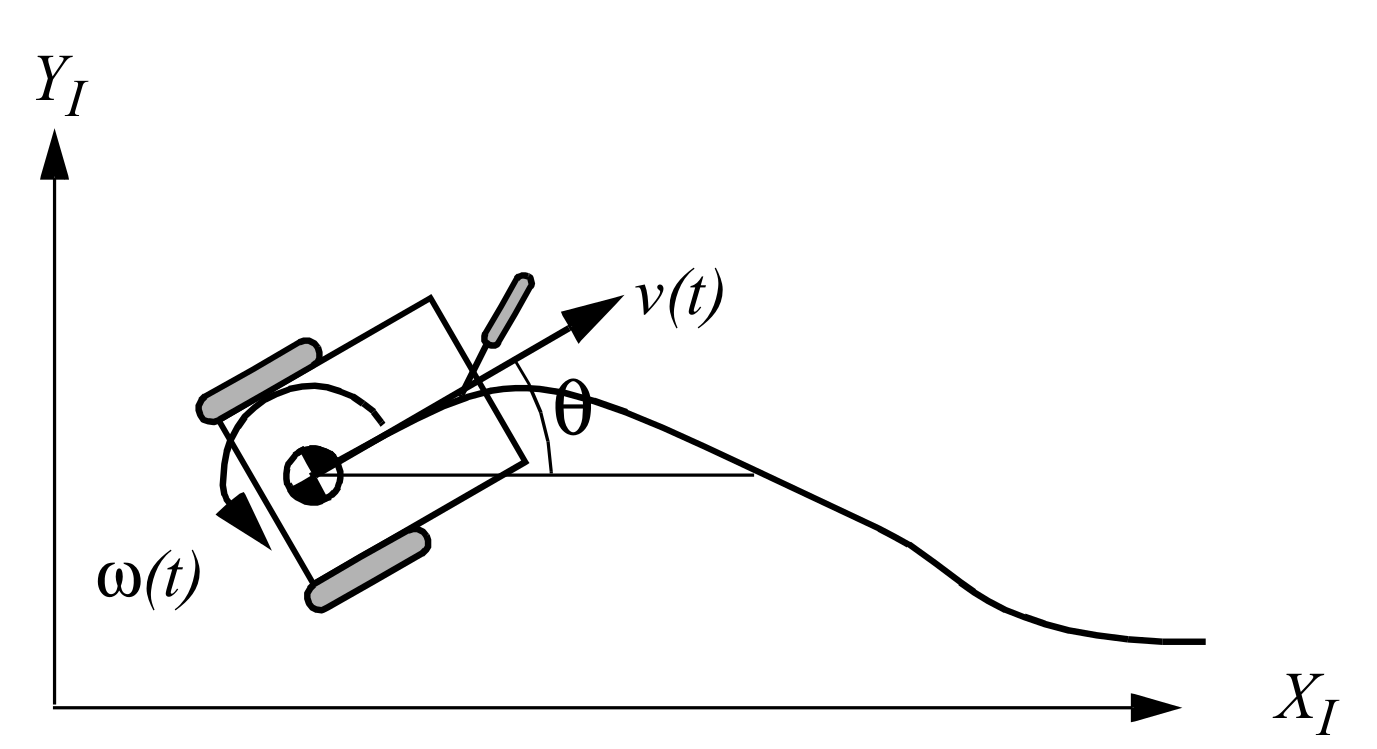
\includegraphics[scale=0.9]{figuras/robo.png}
    \caption[]{Robô móvel com acionamento diferencial}
\end{figure}

A cinemática de um robô móvel está fortemente relaciona a modelagem
das rodas do robô, de forma geral chega-se os seguintes sistemas
afim: $L_r\times v_r +B_r = \phi_r$ e $K_r \times v_r + C_r = 0$

\[
\begin{bmatrix}
    A_{11}sen(W_{11}\alpha_{11} + \beta_{11}) &  A_{12}sen(W_{12}\alpha_{12} + \beta_{12}) &  A_{13}sen(W_{13}\alpha_{13} + \beta_{13})\\
    A_{21}sen(W_{21}\alpha_{21} + \beta_{21}) &  A_{22}sen(W_{22}\alpha_{22} + \beta_{22}) &  A_{23}sen(W_{23}\alpha_{23} + \beta_{23})\\
    \vdots & \vdots & \vdots \\
    A_{n1}sen(W_{n1}\alpha_{n1} + \beta_{n1}) &  A_{n2}sen(W_{n2}\alpha_{n2} + \beta_{n2}) &  A_{n3}sen(W_{n3}\alpha_{n3} + \beta_{n3})\\
\end{bmatrix}
\begin{bmatrix}
    v_x \\
    v_y \\
    \omega\\
\end{bmatrix}
+
\begin{bmatrix}
    B_0 \\
    B_1 \\
    \vdots \\
    B_n \\
\end{bmatrix}
=
\begin{bmatrix}
    \phi_0 \\
    \phi_1 \\
    \vdots \\
    \phi_n \\
\end{bmatrix}
\]
\newpage

\[
\begin{bmatrix}
    D_{11}sen(Q_{11}\gamma_{11} + \mu_{11}) &  D_{12}sen(Q_{12}\gamma_{12} + \mu_{12}) &  D_{13}sen(Q_{13}\gamma_{13} + \mu_{13})\\
    D_{21}sen(Q_{21}\gamma_{21} + \mu_{21}) &  D_{22}sen(Q_{22}\gamma_{22} + \mu_{22}) &  D_{23}sen(Q_{23}\gamma_{23} + \mu_{23})\\
    \vdots & \vdots & \vdots \\
    D_{n1}sen(Q_{n1}\gamma_{n1} + \mu_{n1}) &  D_{n2}sen(Q_{n2}\gamma_{n2} + \mu_{n2}) &  D_{n3}sen(Q_{n3}\gamma_{n3} + \mu_{n3})\\
\end{bmatrix}
\begin{bmatrix}
    v_x \\
    v_y \\
    \omega\\
\end{bmatrix}
+
\begin{bmatrix}
    C_0 \\
    C_1 \\
    \vdots \\
    C_n \\
\end{bmatrix}
=
\begin{bmatrix}
    0 \\
    0 \\
    \vdots \\
    0 \\
\end{bmatrix}
\]
onde $A$, $D$, $W$, $Q$, $B$, $C$, $\alpha$, $\gamma$, $\beta$, $\mu$
são propriedades das rodas do robô. $v_x$,$v_y$ são as velocidade lineares
do robô  e $\omega$ é a velocidade angular do robô.  É importante salientar
que os parâmetros das rodas são extraídos seguindo o referencial do robô $X_r$,$Y_r$.
Caso a velocidade linear do robô for medida em outro referencial, é necessário
fazer uma rotação do referencial medido para a orientação do robô
\begin{figure}[H]
    \centering
    % 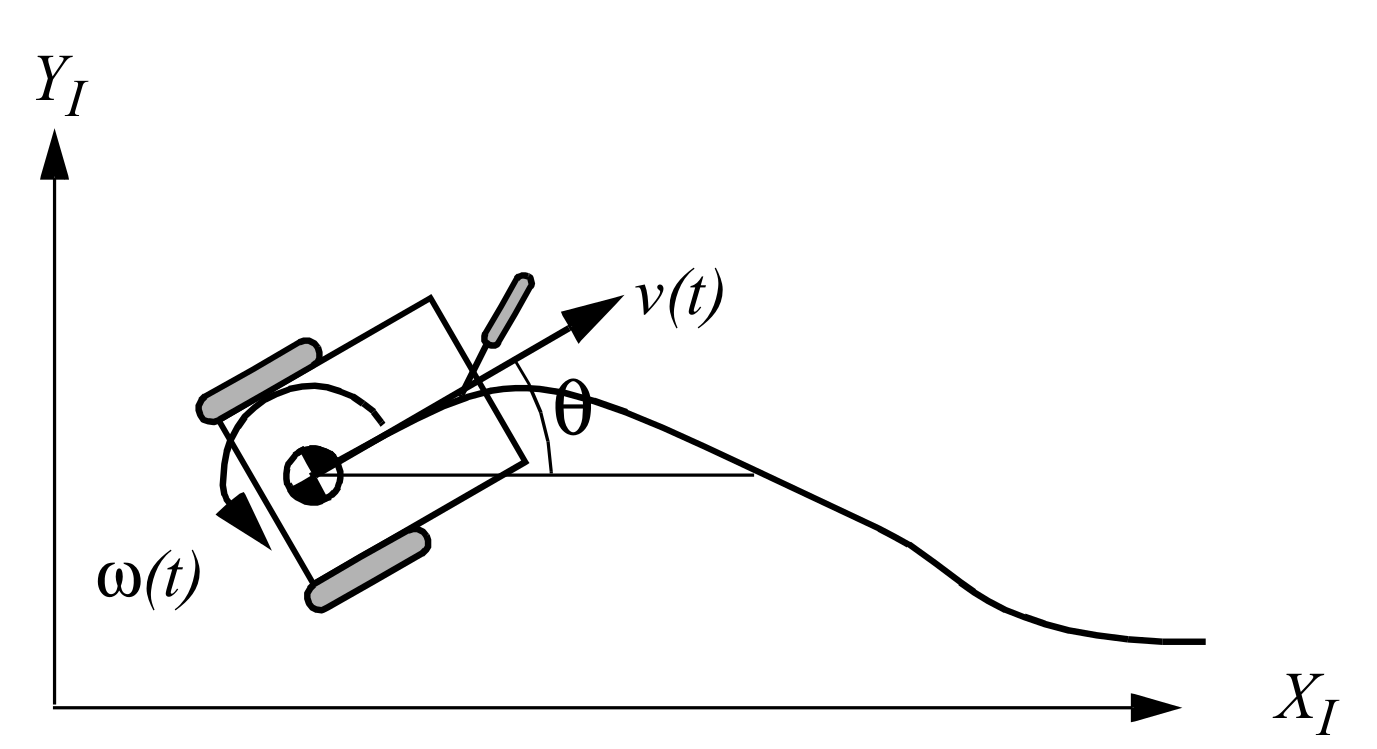
\includegraphics[scale=0.9]{figuras/robo.png}
    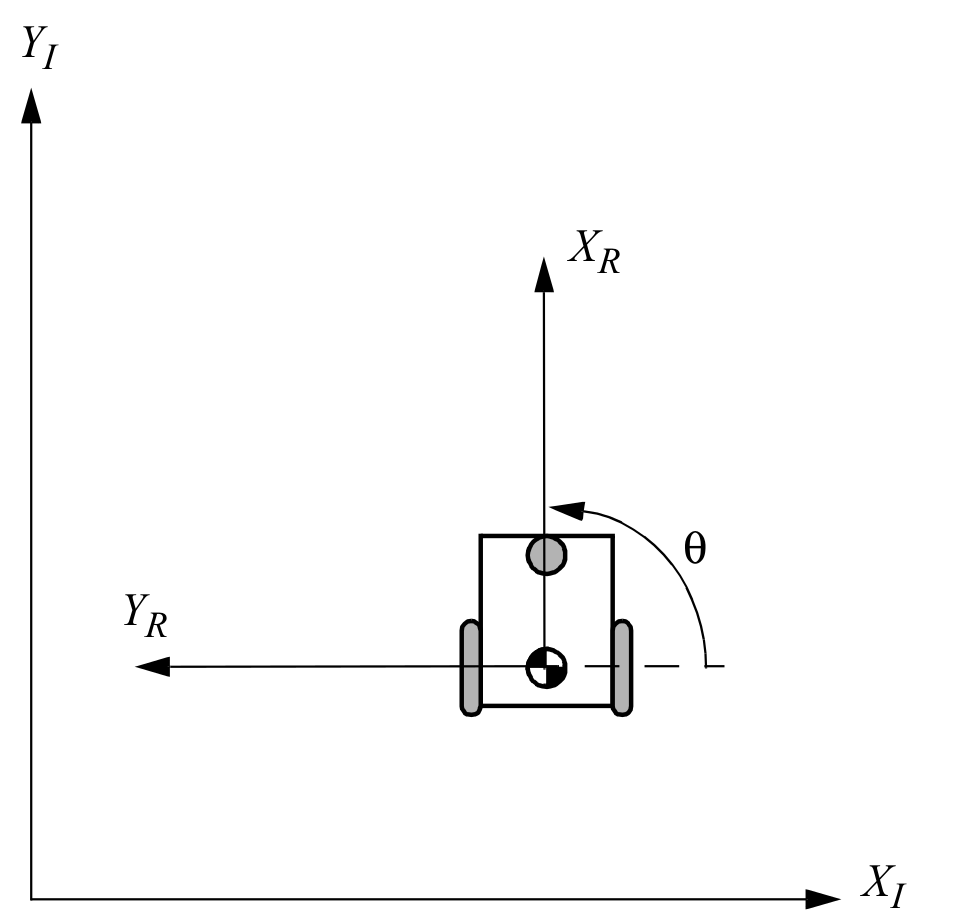
\includegraphics[scale=0.3]{figuras/robo_coordenadas.png}
    \caption[]{Mudança de referencial}
\end{figure}

\[
    \begin{bmatrix}
        v_x \\
        v_y \\
        \omega
    \end{bmatrix}
    =
    \begin{bmatrix}
        cos(\theta)  & sin(\theta) & 0 \\
        -sin(\theta) & cos(\theta) & 0 \\
        0 & 0 & 1 \\
    \end{bmatrix}
    \begin{bmatrix}
        v_{x_I} \\
        v_{y_I} \\
        \omega
    \end{bmatrix}
\]

onde $v_{x_I}, v_{y_I}$, são as velocidades no referencial $X_I,Y_I$.
\newpage

No nosso caso, o robô a ser modelado possui quatro rodas, duas delas são
rodas tratore e as outras duas rodas, são rodas castores. Apesar das rodas
castores, contribuírem para o movimento, elas não restringem o movimento,
portanto podemos entender o modelo cinemático do nosso robô como sendo
uma transformação afim $W \times X + B = Y$, onde $X$ são as entradas
do nosso modelo cinemático, $W$ e $B$ são parâmetros das
rodas que devido a modelagem e a construção do robô, são parâmetros
constantes. No nosso robô, caso queremos calcular a cinemática direta
a entrada $X$ são as velocidades das rodas do robô e $Y$ a velocidade
linear e angular do robô, caso queiramos calcular a cinemática inversa
do robô, $X$ são as velocidades lineares e a velocidade angular do robô
e $Y$ as velocidades da rodas. Neste trabalho visamos criar um controlador
para o robô e como o controlador enviará um sinal de velocidade linear
e angular para a cinemática, portanto queremos a cinemática inversa
do nosso robô.

\begin{figure}[H]
    \[
    \begin{bmatrix}
        W_{11} &  W_{12} & W_{13} \\
        W_{21} &  W_{22} & W_{23} \\
    \end{bmatrix}
    \begin{bmatrix}
        v_x \\
        v_x \\
        \omega \\
    \end{bmatrix}
    +
    \begin{bmatrix}
        B_{1} \\
        B_{2} \\
    \end{bmatrix}
    =
    \begin{bmatrix}
        \phi_{\text{left}} \\
        \phi_{\text{right}} \\
    \end{bmatrix}
\]
    \caption{Cinemática inversa}
\end{figure}


\begin{figure}[H]
    \centering
    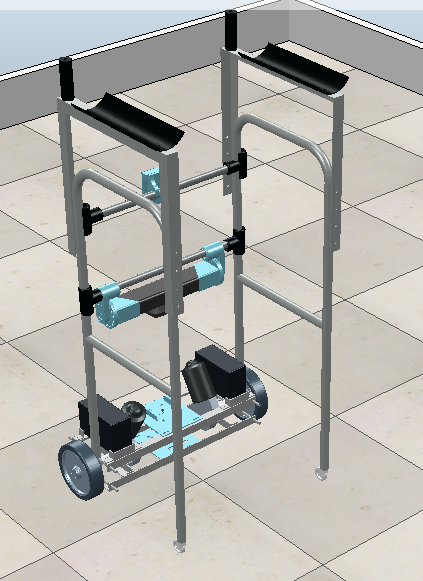
\includegraphics[scale=0.4]{figuras/smart_walker.png}
    \caption{Andador inteligente}
\end{figure}

\section{Aprendizado de máquina}
Usualmente quando programamos computadores para
resolver determinada tarefa, nos codificamos as regras e
executamos o programa com os dados de entrada, esta é a abordagem clássica
de se resolver um problema. Uma outra forma de usar computadores
é criar sistemas como aprendizado máquina, onde nós possuímos os
dados de entrada necessários, as respontas e queremos que a máquina retorne
para nós quais são as regras que transformam os dados nas respostas
desejadas \cite{chollet2021deep}.

\begin{figure}[H]
    \centering
    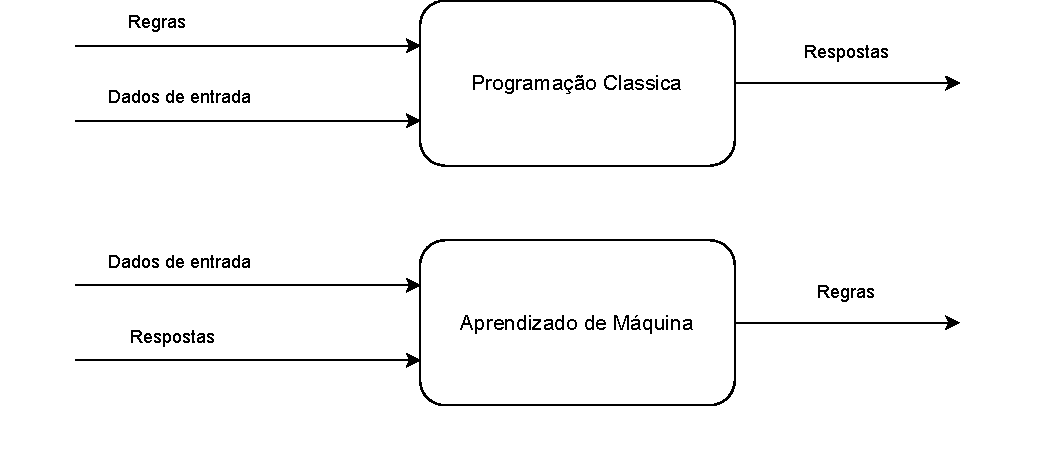
\includegraphics[scale=0.7]{figuras/machine_learning_diagram.pdf}
    \caption{Aprendizado de máquina e Programação clássica}
\end{figure}

Existem três tipos de aprendizado de máquina, aprendizado por reforço,
aprendizado supervisionado e aprendizado não supervisionado.
Aprendizado por reforço é o aprendizado de como mapear situações
para ações de modo que maximize um sinal de recompensa
\cite{sutton2018reinforcement}. Aprendizado supervisionado é o
tipo de aprendizado onde a máquina busca extrair padrões nos conjuntos
de dados de entrada  e do conjunto de dados das respontas de modo que
transforme um dado de entrada na resposta desejada, já aprendizado não
supervisionado também buscar encontrar padrões entre os conjuntos de
dados de entrada e resposta, mas sem ter uma responta correta
\cite{trask2019grokking}. Neste trabalho foi utilizado algoritmos de
aprendizado de máquina supervisionado com objetivo de extrair um modelo de
cinemática inversa do robô andador inteligente.

\begin{figure}[H]
    \centering
    \includegraphics[scale=0.7]{figuras/aprendizado_cinemática_inversa.pdf}
    \caption{Aprendizado de máquina no calculo da cinemática inversa}
\end{figure}

Os algoritmos de aprendizado supervisionado utilizado neste trabalho
foram o Backpropagation e uma variação do algoritmo decida do gradiente, chamada
RMSprop.
Dado uma função $L(M)$, onde $L$ é uma função continua e derivável,
a decida do gradiente é uma busca que visa encontrar
a melhor matriz $M$ que minimiza uma função $L(M)$, basicamente a
decida do gradiente parte do suposto que existe a sequência
$M_0$, $M_1$, $M_2$, ..., $M_i$, $M_{i+1}$ até $M_k$, onde quando
chegar até $M_k$, o erro $L(M_k)$ será um ponto de mínimo e a transição
entre o $M_{i}$ até $M_{i+1}$, segue a seguinte regra:

\begin{figure}[H]
    \[
        M_{i+1} = M_i -\alpha \nabla L(M_i)
    \]
    \caption{Equação da decida do gradiente}
\end{figure}

onde $\nabla L(W)$ é o gradiente da função erro em relação $M$ aplicado
a $M_i$ e $\alpha$ é um número que varia de 0 até 1,
também conhecido com taxa de aprendizado. Uma variação desse algoritmo
basicamente utilizado é chamado RMSprop, ele se inspira na ideia de momentum
da física  onde  é adicionado uma constante $m$ análoga a massa e uma grandeza
vetorial $v_{\text{vel}}$ análoga a velocidade, criando uma nova equação de decida:

\begin{figure}[H]
    \begin{align*}
        v_{\text{vel}_t} = \alpha v_{\text{vel}_{t-1}} + (1 - \alpha)\nabla L(M_i)^2 \\
        b_t = mb_{t-1} + \frac{\nabla L(M_i)}{\sqrt{v_{\text{vel}_t} + \epsilon}} \\
        M_{i+1} = M_i - b_t
    \end{align*}
    \caption{Equações do RMSprop}
\end{figure}

As variáveis $v_{\text{vel}_t}$ e  $b_t$, são inicializadas como zero, pode acontecer
que  $\sqrt{v_{\text{vel}_t}}$ seja zero ou bem próximo disso então para não ter uma equação
divida por zero é adicionado uma variável $\epsilon =10^{-8}$, deixando o algoritmo numericamente
mais estável. Em contexto de aprendizado supervisionado a função $L$ é uma função erro que a
partir do Backpropagation, encontra-se os gradientes dos parâmetros de um modelo a partir
de pontos $X$ e $Y$ coletados, partindo de  uma definição de um modelo como por exemplo uma
transformação geométrica $Y_{\text{pred}}= A \times X + B$, e uma definição de uma função
erro como: $L=(Y_{\text{true}}- Y_{\text{pred}})^2$ podemos utilizar o algoritmo
Backpropagation para encontrar os gradientes da função $L$ em relação a $A$
e  $B$, basicamente o Backpropagation executa automaticamente a regra da cadeia
para encontrar os gradientes e com os gradientes podemos executar o RMSprop.

\begin{figure}[H]
    \begin{align*}
        \frac{dL}{dA } = \frac{dL}{dY_{\text{pred}} } \frac{dY_{\text{pred}}}{dA}  \\
        \frac{dL}{dB } = \frac{dL}{dY_{\text{pred}} } \frac{dY_{\text{pred}}}{dB} 
    \end{align*}
    \caption{Regra da cadeia aplicada ao modelo: $Y_{\text{pred}}= A \times X + B$ }
\end{figure}



\section{Controlador estabilizante Federico}
Controladores cinemáticos ou controladores de movimento, podem ser 
divididos em dois tipos, seguidores de trajetória e retroalimentação,
controladores seguidores trajetória recebem como entrada um perfil
de caminho sobre o tempo, a qual o controlador envia sinais de
velocidade linear e angular para o robô de modo que ele siga a
trajetória idealizada, já controladores de retroalimentação
eles recebem como entrada um estado atual do robô e o estado desejado
e buscam enviar sinais de velocidade linear e angular com o objetivo
de minimizar o erro entre o estado atual e desejado. Neste trabalho
foi utilizado um controlador de retroalimentação criado por Frederico
\cite{vieira2006controle}, o controlador recebe como entrada a posição
x,y $p_c$, orientação $\theta_c$ atual do robô e uma posição desejada $p_d$
e enviar sinais de velocidade linear $v$ e angular $\omega$ com o
objetivo de estabilizar o robô no ponto desejado.

\begin{figure}[H]
    \centering
    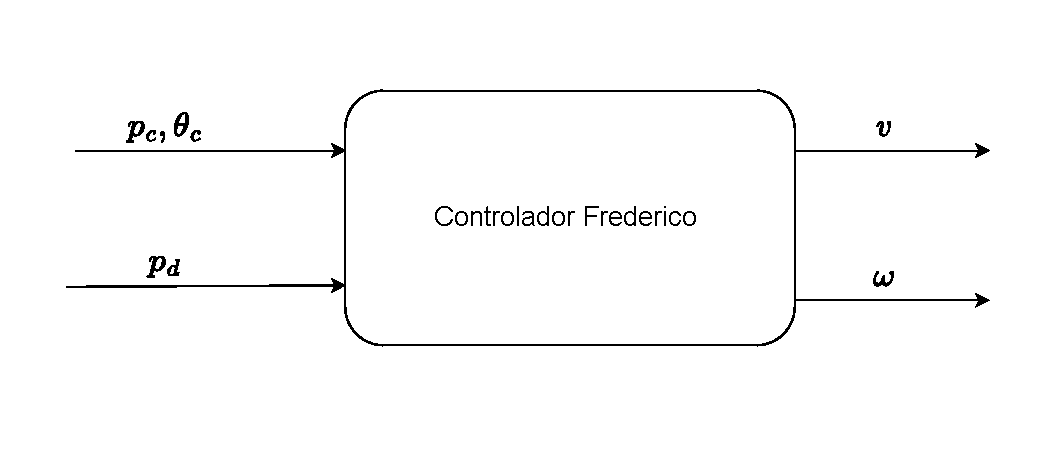
\includegraphics[scale=0.8]{figuras/controlador_frederico.pdf}
    \caption{Bloco controlador Frederico}
\end{figure}

Internamente o controlador utiliza  dois controladores proporcionais
integrais derivativos (P.I.D), um controlador é responsável pela velocidade linear $v$
e outro controlador é responsável pela velocidade angular $\omega$. 
Um controlador P.I.D é definido pela a seguinte função de
transferência $C(s)$ no domínio continuo $s$

\begin{figure}[H]
    \[
        C(s) = K_p + \frac{K_i}{s} + K_ds
    \]
    \caption{Função de transferência de um controlador P.I.D }
\end{figure}
onde $K_p$,$K_i$,$K_d$ são constantes que podem ser adquiridas ou
através da experimentação ou uma analise matemática. Para gerar sinais
velocidades $v$ e $\omega$,  o controlador Federico funciona da seguinte
maneira, primeiro é calculado o vetor posição $p_{\text{diff}}$:
\[
    p_{\text{diff}} = p_d - p_c 
\]
segundo é calculado suas coordenadas polares $l$, $\alpha$:

\[
    l = \sqrt{p_{\text{diff}_x}^2 + p_{\text{diff}_y}^2}
\]

\[
    \alpha =  \arctan(\frac{ p_{\text{diff}_y}}{p_{\text{diff}_x}}) 
\]

onde $p_{\text{diff}_x}$,$p_{\text{diff}_y}$ são as coordenadas x,y
do vetor $p_{\text{diff}}$. Terceiro é calculado o angulo $\gamma$:

\[
    \gamma =  \alpha - \theta
\]


por fim o controlador P.I.D de velocidade
linear, buscar enviar um sinal $v$ que para tender o valor $l \cos(\gamma)$
a zero e o controlador de velocidade angular busca enviar um sinal $\omega$
para  tender o valor de $\gamma$ a zero. perceba que quando o valor de $\gamma$
chega próximo a zero, da velocidade linear vai tender a reduzir a
distância $l$. Como o modelo cinemático do robô espera receber como entrada
um vetor de velocidade linear em coordenadas cartesianas então é preciso
transformar de volta a velocidade $v$ 

\[
    \begin{bmatrix}
        v_x \\
        v_y \\
    \end{bmatrix}
    =
    \begin{bmatrix}
        v\cos(\theta) \\
        v\sin(\theta) \\
    \end{bmatrix}
\]
onde, $v_x$, $v_y$ são as velocidade lineares em coordenadas cartesianas.

% Cap. 3 - Trabalhos Relacionados
%%
%% Capítulo 2: Expressões matemáticas
%%

\mychapter{Trabalhos relacionados}
\label{Cap:TrabalhosRelacionados}
Neste capítulo abordaremos os três principais artigos que influenciaram
este trabalho. O primeiro artigo se trata de um algoritmo do estado
da arte do aprendizado por reforço, o segundo e terceiro artigo são
trabalhos que buscaram criar um controlador usando aprendizado por reforço
que rivaliza com os controladores que utilizam a abordagem clássica de controle.
Estes dois últimos artigos foram determinantes para escolher o controlador
de estabilizante Vieira. Para este trabalho a parte fundamental do primeiro artigo
foi resumida na seção \ref{sec:muzero}. A forma como os outros dois artigos
utilizaram aprendizado por reforço para criar um controlador de posição e seus
resultados foi escrita na seção \ref{sec:controlador:posicao:aprendizado:reforco}.
Por último a conclusão que me levou a utilizar o controlador estabilizante Vieira
foi escrita na seção \ref{sec:conclusao:revisao:bibliografica}.

\section{MuZero}
\label{sec:muzero}

MuZero é um sistema de aprendizado de máquina que utiliza algoritmos de
aprendizado por reforço e aprendizado supervisionado para
resolver jogos de atari, xadrez e Shogi também conhecido como
xadrez japonês. O MuZero é um sistema com três componentes:
Representação, dinâmica e predição, Representação é uma uma
função $h_{\theta}$  que recebe $t$ observações 
e cria uma Representação interna $s$, $s = h_{\theta}(o_1,...,o_t)$,
onde $o$ é uma observação, onde uma observação pode ser entendia como sendo
um vetor que contem todos os valores dos sensores em um instante $t$.
A predição é uma função $f_{\theta}$ que recebe uma representação $s$
e retorna uma vetor de valores $v[k]$ que dizem o quão boa seria tomar
uma decisão discreta $k$,  $v[k] =  f_{\theta}(s)$ ,
para cada ação discreta $k$, uma ação $a$, poderia ser o índice do maior
valor de $v[k]$ ou utilizar a busca em árvore como no método Monte Carlo
através do modelo de dinâmica. O modelo de dinâmica é uma outra função
$g_{\theta}$, que busca prever dado uma ação $a^k$ e um estado $s^{k}$,
o estado $s^{k+1}$ e sua recompensa $r^{k+1}$ associada ao estado,
ou seja, $s^{k+1},r^{k+1}=  g_{\theta}(s^{k},a^k)$.


\begin{figure}[H]
    \centering
    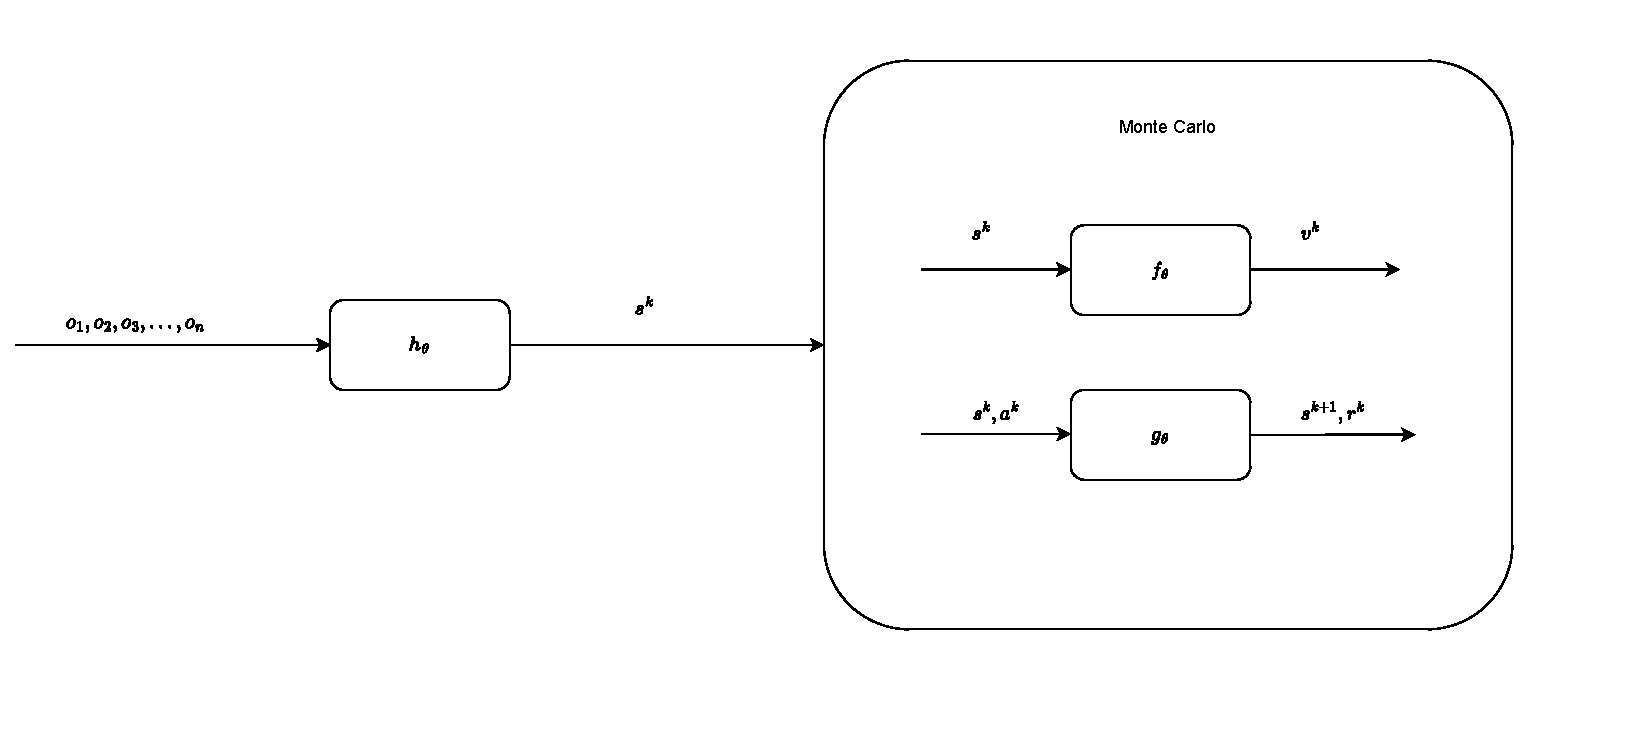
\includegraphics[scale=0.4]{figuras/muzero.pdf}
    \caption{diagrama dos modelos do Muzero}
\end{figure}

A importância do MuZero para este trabalho não se trata do modelo em si,
mas sim a forma como resolveu o problema, dividindo o sistema em componentes
de forma muito semelhante a como é feito em teoria de controle, onde
o modelo de predição  $f_{\theta}$ pode ser entendido algo
análogo ao controlador, o  modelo dinâmico $g_{\theta}$ como a planta,
e $h_{\theta}$ sendo os sensores, sendo $h_{\theta}$ o modelo
necessário  para que o sistema seja genérico o suficiente para jogar
diferentes jogos. É importante destacar a diferença entre o controlador P.I.D
que toma decisões a partir de $n$ instantes anteriores ($t_n,t_{n-1},...t_{0}$),
já o $f_{\theta}$
com a buscar Monte Carlo toma decisões em $k$ instantes futuros ($t_n,t_{n+1},...t_{n+k}$)
utilizando a função $g_{\theta}$ análoga á planta.

\begin{figure}[H]
    \centering
    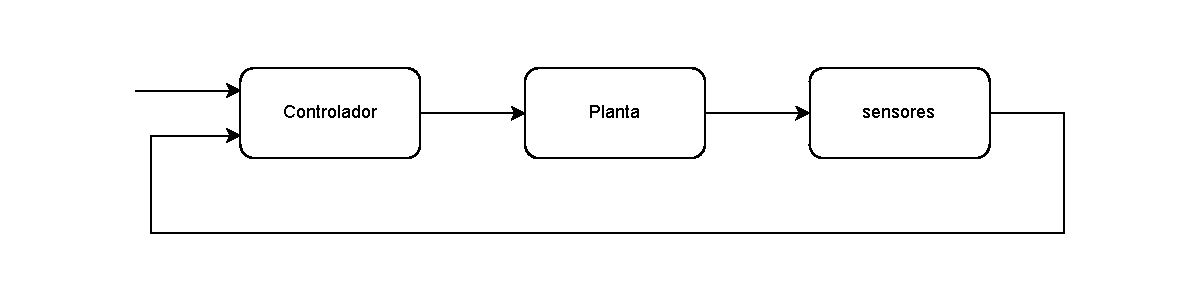
\includegraphics[scale=0.6]{figuras/sistema_classico_controle.pdf}
    \caption{diagrama clássico de controle}
\end{figure}

\section{Controlador de posição e aprendizado por reforço }
\label{sec:controlador:posicao:aprendizado:reforco}
Utilização de aprendizado por reforço para criação de controladores
de estabilizante, foi observado em \cite{farias2020position}
a qual mostrou que o algoritmo \textit{Q-learning} é capaz de aprender
as regras de um controlador com restrições de velocidades linear e angular
para  posicionar o robô em determinada posição, no entanto em seus
experimentos foram necessários 5 milhões de iterações para se ter um modelo
inferior a um controlador que utiliza as leis clássicas de controle.

\subsection{Q-learning}
Uma Função ação-valor determina o quão bom 
para o robô é tomar uma determinada ação $A_t$ quando se está no estado
$S_t$, \textit{Q-learning} é um algoritmo de aprendizado por reforço que
busca aprender uma função ação-valor $Q$ que diretamente aproxima
a função ação-valor ótima $Q^*$ independente do algoritmo utilizado
para selecionar uma ação. O que faz o algoritmo aproximar a função ótima
é o processo de atualização da função $Q$ seguindo a equação do \textit{Q-learning}:

\begin{equation} 
    Q(S_t,A_t) \leftarrow Q(S_t,A_t) + \alpha[R + \gamma  \max_aQ(S_{t +1},a) - Q(S_t,A_t)]
\end{equation}
onde $S_t$ e $A_t$ é respectivamente estado,ação, $\max_aQ(S_{t +1},a)$ é o valor da
ação de maior valor no estado $S_{t+1}$ e as constantes $\alpha$, $\gamma$ são taxas
de aprendizado que variam de 0 até 1. É muito comum representar a função $Q$
sendo como uma tabela, onde o estado $S$ e ação $A$ são indices. Em contexto de
controladores de estabilizante para robôs moveis, o estado pode ser um
valor de distância até o alvo discretizado e ação pode ser movimentos simples
como girar para esquerda, direita, ir para frente ou ir de rê. Por fim o valor é
número contínuo ou discreto derivado de uma função recompensa que poder
a a variação de distância até o alvo observada após o movimento.
\textit{Q-learning} é apresentado em Algoritmo  \ref{Q-learning:}


\begin{algorithm}[H]
    \label{Q-learning:}
    Parâmetros dos algoritmo: importância de um passo $\alpha \in (0,1]$
    taxa de aprendizado $\gamma \in (0,1] $

    
    \Entrada{ número de epsodios $N_e$; número de passos $N_p$ }
    %% \SetLine
    
    inicialize $Q(s,a)$ arbitrariamente exceto $Q(\text{terminal},\cdot ) = 0$

    \Para {$e \leftarrow 0$ \Ate $N_e$} {
        inicialize o $S$ com o estado inicial $S_0$

        
        \Para {$j \leftarrow 0$ \Ate $N_p$} {
            Escolha a ação $A$ do estado $S$ usando alguma regra derivada de $Q$,
            por exemplo a $\epsilon$-greedy

            Realize a ação $A$ e observe a recompensa $R$ e o novo estado $S'$
            
            $Q(S,A) \leftarrow (S,A) + \alpha[R + \gamma \max_aQ(S',a) - Q(S,A)]$
            
            $S \leftarrow S'$


            \Se {S é terminal}{
                
              $j \leftarrow N_p$  \textbf{ fim do loop de passos}
            }
        }
        
    }
    \Retorna $Q(s,a)$
    \caption{Algoritmo Q-learning}
    
\end{algorithm}

Em \cite{quiroga2022position}
foram utilizado algoritmos variantes do \textit{Q-learning},
como \textit{Deep Q-learning Network} e \textit{Deep Deterministic Policy Gradient},
para encontrar as regras de um controlador que posicione o robô em determinada
posição e evite de obstáculos usando sensores ultrassônicos,
apesar do sucesso, o controlador gerado pelos algoritmos não envia
os sinais de velocidades angulares diretamente para o modelo cinemático
do robô, os sinais eram a entrada para o algoritmo de Braitenberg, um
algoritmo que converte sinais de distância de obstáculos em velocidades
lineares e angulares de modo que evite a colisão com obstáculos, além do treinamento permitir que o robô
colida com o obstáculo, foi observado que o tempo de treinamento desses modelos
foram de 8,6 e 11,4 horas de treinamento para \textit{Deep Q-learning Network}
e \textit{Deep Deterministic Policy Gradient}, respectivamente. Segundo o
artigo o melhor o controlador foi o \textit{Deep Deterministic Policy Gradient}
que conseguiu chegar na posição desejada 3 segundos mais rápido do que o
melhor controlador que utiliza as leis clássicas de controle isso em um ambiente sem
obstáculos e em um ambiente com obstáculos a diferença aumentou para
17,3 segundos, no entanto a distância do robô até os obstáculos ficou
inferior a 20 centímetros, ou seja, o modelo de aprendizado encurtou o
caminho ficando mais próximo de bater no obstáculo. É importante dizer que
em ambos os trabalhos foi utilizado um robô de acionamento diferencial.

\subsection{Deep Q-learning e Deep Deterministic Policy Gradient }
\textit{Deep Q-learning Network} é o algoritmo \textit{Q-learning}
aplicado a redes neurais de modo que a função gerada pelo treinamento
dessa rede é uma aproximação da função valor ótima $Q^*$, uma das vantagens
de utilizar redes neurais é o fato de poder utilizar estados contínuos sem a
necessidade de discretização, no entanto o espaço de ação ainda é necessário
ser discreto. Muitas das vezes esse algoritmo é utilizado
tendo como estado $S$ sendo uma imagem que normalmente é preprocessada
antes de enviada para a rede neural. Para ter um treinamento mais estável,
são utilizados duas redes, onde a rede alvo é atualizada usando o parâmetro
de polyak $\rho$ após o fim de uma época $e$.
O algoritmo do \textit{Deep Q-learning Network}
pode ser vista no Algoritmo \ref{Deep:Q-learning:}

\begin{algorithm}[H]
    %% \SetLine
    Parâmetros dos algoritmo:
    importância de um passos $\alpha \in (0,1]$,
    taxa de aprendizado $\gamma \in (0,1]$,
    polyak $\rho \in (0,1]$,
    capacidade da memória $C \in \mathbb{N}$
    tamanho do minibatch $K \in \mathbb{N}$

    \Entrada{ número de epsodios $N_e$; número de passos $N_p$ }

    inicialize os pesos $\theta$ da rede neural que aproxima a função $Q$ com valores aleatórios

    inicialize os pesos $\theta_{\text{target}}  \leftarrow \theta$ rede alvo $Q_{\text{target}}$

    \Para {$e \leftarrow 0$ \Ate $N_e$} {
        inicialize a sequencia $s_0$

        inicialize a sequência preprocessada $\phi_0 \leftarrow \phi(s_0)$ 
        

        \Para {$j \leftarrow 0$ \Ate $N_p$} {
            Escolha a ação $a_t$ do estado processado $phi_t$ usando alguma regra derivada de $Q$,
            por exemplo a $\epsilon$-greedy

            Realize a ação $a_t$ e observe a recompensa $r_t$ e o nova imagem $x_{t+1}$
            
            $s_{t+1}  \leftarrow (s_t, a_t, x_{t+1})$   

            preprocesse a sequencia $\phi_{t+1} \leftarrow \phi(t+1)$
            
            armazene a transição $(\phi_t,a_t,r_t,\phi(t+1))$ na memória $M$

            \Se {$K \ge$ total de transições armazenadas}{
                Selecione $K$ amostras para formar um minibatch de transições

                inicialize o conjunto $y$ de valores desejados
    
                \Para {$k \leftarrow =0$ \Ate $K$}{
    
    
                    \eSe {$s_k$ é terminal}{
                    
                        $y_k \leftarrow r_k$
                      }
                      {
                        $y_k \leftarrow r_k + \gamma \max_aQ(\phi_k,a_k)$
                      }
                    
                }
    
                atualize os pesos $\theta$ baseado no erro $\frac{1}{|K|} \sum_{b =0}^{K}(y -Q(\phi_b,a_b))^2$

        
            }

            \Se {$s_{t+1}$ é terminal}{
                
                $j \leftarrow N_p$  \textbf{ fim do loop de passos}
              }

        }

        ao fim de uma época, atualize os pesos da rede alvo
        $\theta_{\text{target}}  \leftarrow \rho \theta_{\text{target}}  + (1-\rho) \theta$
        
    }
    \Retorna a rede neural $Q_{\text{target}}$
    \caption{Algoritmo Deep Q-learning}
    \label{Deep:Q-learning:}
\end{algorithm}

Como dito anteriormente o espaço das ações do \textit{Deep Q-learning} são discretas,
visando tornar o espaço de ações também contínuas é acrescentando mais
uma rede neural para aproximar a política $\mu$,
desta forma temos um algoritmo baseado na equação \textit{Q-learning} que permite
aprender um sistema de entrada e saída contínua.
\begin{flalign} 
    A_t = \mu(S_t)\\
    Q(S_t,A_t) \leftarrow Q(S_t,A_t) + \alpha[R + \gamma  Q(S_{t +1},\mu(S_{t+1})) - Q(S_t,A_t)]
\end{flalign}
Enquanto temos uma rede neural $Q$ que busca encontrar a função ação-valor ótima $Q^*$, temos uma
nova rede neural que através do gradiente ascendente buscar encontrar a
política $\mu$ que maximiza a recompensa da função valor aproximada
$Q(S,\mu(S))$.
Perceba que devido a forma como estamos otimizando a rede neural $\mu$,
então o $\max_aQ(S_t,a_k)$ é análogo a $Q(S_t,\mu(S_t))$.
O algoritmo do \textit{Deep Deterministic Policy Gradient}
pode ser vista no Algoritmo \ref{Deep Deterministic Policy Gradient:}. Ambos os
algoritmos \textit{Deep Q-learning} e \textit{Deep Deterministic Policy Gradient} 
foram retirados da documentação da \textit{OpenIA} \cite{SpinningUp2018}, salvo pequenas
adaptações.

\begin{algorithm}[H]
    %% \SetLine
    Parâmetros dos algoritmo:
    importância de um passo $\alpha \in (0,1]$,
    taxa de aprendizado $\gamma \in (0,1]$,
    polyak $\rho \in (0,1]$,
    capacidade da memória $C \in \mathbb{N}$
    tamanho do minibatch $K \in \mathbb{N}$ 

    \Entrada{ número de epsodios $N_e$; número de passos $N_p$ }

    inicialize a memória $M$ com a capacidade $C$

    inicialize os pesos $\theta$ da rede neural que aproxima a função $Q$ com valores aleatórios

    inicialize os pesos $\theta_\mu$ da rede neural que a aproxima da política $\mu(\phi)$ com valores aleatórios

    inicialize os pesos $\theta_{\text{target}}  \leftarrow \theta$ rede alvo $Q_{\text{target}}$

    inicialize os pesos $\theta_{\mu_{\text{target}}}  \leftarrow \theta_\mu$ rede alvo $\mu_{\text{target}}$


    \Para {$e \leftarrow 0$ \Ate $N_e$} {
        inicialize a sequencia $s_0$

        inicialize a sequência preprocessada $\phi_0 \leftarrow \phi(s_0)$ 
        

        \Para {$j \leftarrow 0$ \Ate $N_p$} {
            Escolha a ação $a_t$ do estado processado $phi_t$ usando a rede  $\mu(\phi) + \epsilon$, onde
            $\epsilon$ é um ruído que controla a exploração, $a_t \leftarrow \mu(\phi_t)  + \epsilon$ 

            Realize a ação $a_t$ e observe a recompensa $r_t$ e o nova imagem $x_{t+1}$
            
            $s_{t+1}  \leftarrow (s_t, a_t, x_{t+1})$   

            preprocesse a sequencia $\phi_{t+1} \leftarrow \phi(t+1)$
            
            armazene a transição $(\phi_t,a_t,r_t,\phi(t+1))$ na memória $M$

            \Se {$K \ge$ total de transições armazenadas}{
                Selecione $K$ amostras para formar um minibatch de transições

                inicialize o conjunto $y$ de valores desejados
    
                \Para {$k \leftarrow =0$ \Ate $K$}{
    
    
                    \eSe {$s_k$ é terminal}{
                    
                        $y_k \leftarrow r_k$
                      }
                      {
                        $a_d = \mu_{\text{target}}(\phi_k)$
    
                        $y_k \leftarrow r_k + \gamma Q_{\text{target}}(\phi_k,a_d)$
                      }
                    
                }

                atualize os pesos $\theta$ baseado no erro  $\frac{1}{|K|} \sum_{b =0}^{K} (y -Q(\phi_b,\mu(\phi_b)))^2$
                
                atualize os pesos $\theta_\mu$ baseado no gradiente ascendente:
                $\nabla_{\theta_\mu} \frac{1}{|K|} \sum_{b =0}^{K} Q(\phi_b,\mu(\phi_b))$
            
            }

           
        }

        atualize os pesos da rede alvo $\theta_{\text{target}}  \leftarrow \rho \theta_{\text{target}}  + (1-\rho) \theta$

        atualize os pesos da rede alvo $\theta_{\mu_{\text{target}}}  \leftarrow \rho \theta_{\mu_{\text{target}}}  + (1-\rho)\theta_\mu$

        
    }
    \Retorna as redes neurais $Q_{\text{target}}$, $\mu_{\text{target}}$
    \caption{Algoritmo Deep Deterministic Policy Gradient}
    \label{Deep Deterministic Policy Gradient:}
\end{algorithm}


\section{Conclusão da revisão bibliográfica}
\label{sec:conclusao:revisao:bibliografica}
Os artigos demostram que para um problema simples como posicionar ou estabilizar
um robô de acionamento diferencial em um ambiente sem obstáculos ou com
obstáculos simples, as soluções com aprendizado de máquina por reforço
envolvendo variantes de \textit{Q-learning} visando substituir as
leis clássicas de controle não são interessantes, pois usam muito mais
memória, processamento e apresentam resultados equiparáveis quando não
piores que as soluções utilizando leis clássicas de controle. 

% Cap. 4 - Problema
%%
%% Capítulo 4: Desenvolvimento
%%

\mychapter{Desenvolvimento}
\label{Cap:Desenvolvimento}

O principal objetivo desse trabalho é criar um controlador para
um Andador inteligente, sendo este controlador pensado para requerer
pouca memória e processamento, também visa-se estudar e aplicar algoritmos
de aprendizagem de máquina de modo a gerar um modelo cinemático do robô.
O modelo cinemático é o maior desafio deste trabalho, pois como será visto
mais adiante foi utilizado uma abordagem que mescla a solução analítica com
algoritmos de aprendizado de máquina para gerar um modelo de um robô com
acionamento diferencial, outra contribuição deste trabalho é o modelo do
robô simulado, onde o controlador, e o modelo cinemático foram avaliados.
O desenvolvimento do controlador, foi dividindo em quatro partes, a primeira
é a construção da simulação do robô, segunda foi a coleta de dados para
a construção do modelo cinemático, terceira foi  modelado
uma rede neural de modo que seus parâmetros se traduzissem nos parâmetros
da cinemática, quarta e ultima parte conta o desenvolvimento
do pre-processamento dos dados e treinamento do modelo. 


\section{construção do robô em um ambiente simulado}
O simulador utilizado para a construção do robô foi o CoppeliaSim
\cite{rooban2021coppeliasim}, antigamente conhecido como V-REP.
Uma das contrições deste trabalho foi a criação de um cliente 
\textit{zmqRemoteApi} para a linguagem de programação \textit{Rust}
que se comunica com o simulador, \textit{Rust} foi adotado pois
é capaz de produzir um código tão performático quando C/C++, além
de possui um gerenciador de pacotes que facilita o desenvolvimento
futuro de novas aplicações e reutilização de códigos. O ambiente
da simulação é possui o formato quadro com um lado $l$ de 5 metros,
além do robô, o ambiente possui um alvo, a qual o robô deve-se ir
atrás dele, o alvo é um objeto que pode ser movido com mouse. 

\begin{figure}[H]
    \centering
    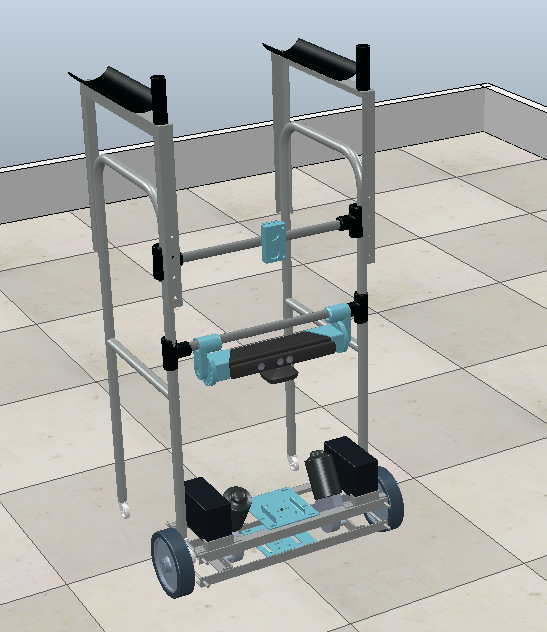
\includegraphics[scale=0.2]{figuras/robo_simulado_1.png}%
    \hspace{1cm}
    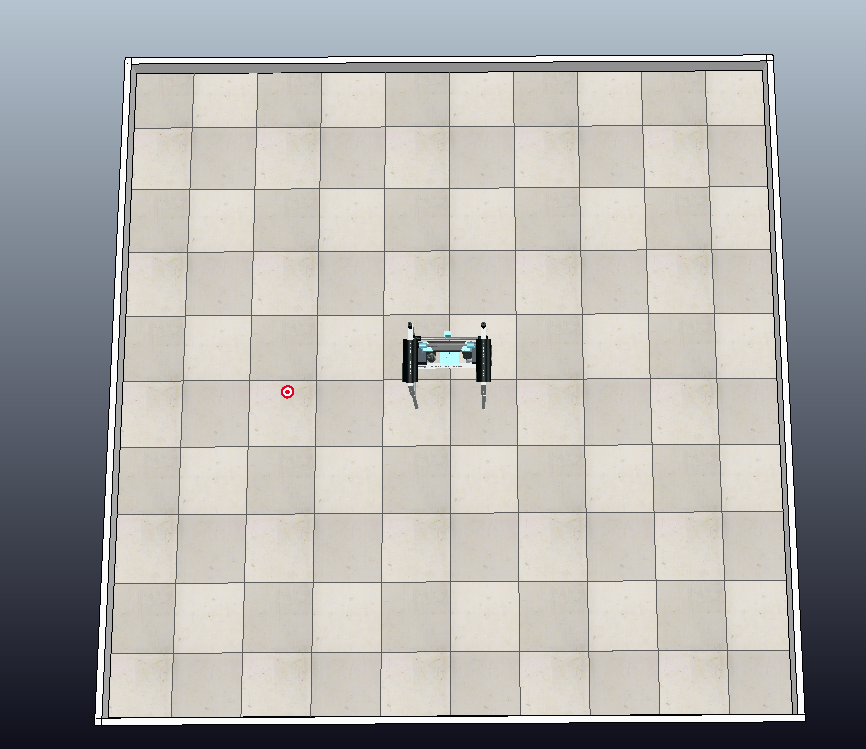
\includegraphics[scale=0.2]{figuras/visao_cima.png}
    \caption{Andador inteligente simulado}
\end{figure}

Como dito anteriormente, o robô possui um acionamento diferencial,
o CoppeliaSim, permite configurar os atuadores no modo controle de
velocidade, neste modo, o cliente \textit{zmqRemoteApi} é capaz de enviar
um sinal em radianos por segundo, a qual é aplicado instantaneamente.


\section{Coleta de dados para o modelo cinemático}
Tendo o robô modelado, a simulação configurada, então foi criado
um algoritmo que faça o robô andar aleatoriamente pelo cenário ao mesmo
tempo que se coletava a posição e orientação do robô em relação ao referencial
global. O pseudo código pode ser observado no Algoritmo \ref{coleta:de:dados:}

\begin{algorithm}[H]
    \label{coleta:de:dados:}
    
    \Entrada{$N_a$:número de amostras, $K$: número de paços continuos }
    %% \SetLine
    
    inicialize a conexão SIM  com o simulador

    inicialize a memória $M$

    mova o robô R para a origem e com uma orientação aleatória $\theta$,
    por meio da conexão SIM

    \Para {$e \leftarrow 0$ \Ate $N_a$} {
        leia a posição $x_1$,$y_1$  e orientação $\theta_{1}$ do robô,
        referente a origem, por meio da conexão SIM
        
        leia o tempo $t_1$ da simulação,por meio da conexão SIM
        
        gere as velocidades das rodas $\phi_l$,$\phi_r$ aleatoriamente,
        entre [0,$V_{MAX}$]
        
        envie  $\phi_l$,$\phi_r$, para o robô simulado pela conexão SIM

        permita que a simulação ocorra por 50ms 

        leia a posição $x_2$,$y_2$  e orientação $\theta_{2}$ do robô,
        referente a origem, por meio da conexão SIM

        leia o tempo $t_2$ da simulação.por meio da conexão SIM

            \Se {$e$ é múltiplo de $K$}{
                
                mova o robô R para a origem e com uma orientação aleatória $\theta$,
                por meio da conexão SIM
            }
        
        armazene em $M$ os valores  ($x_1$,$y_1$,$\theta_{1}$,$t_1$),($x_2$,$y_2$,$\theta_{2}$,$t_2$)
        
    }

    armazene $M$ em um arquivo
    
    \caption{Algoritmo de Coleta de dados}
    
\end{algorithm}

O parâmetro $K$ do algoritmo foi criado para que o robô não bata na parede
da simulação, ele foi encontrado fazendo um teste empírico, mostrando que
após 20 paços  com o robô caminhando em linha reta, o robô bate na parede,
por tanto nos nossos testes $K = 18$. Um princípio foi adotado na coleta
de dados: o robô deve-se mover lentamente em todas a direções, sabendo do
fato que a velocidade linear máxima do robô é 0,8 metros por segundo,
por tanto foi adotado que velocidade linear máxima da coleta seria de 
0,165 metros por segundo, esse número foi adotado por ser significantemente,
inferior a 0,8  e ser o dobro do raio das rodas, ou seja, na prática é gerado
dois números aleatórios de distribuição uniforme entre 0 e 1 e multiplicado por
2, $V_{MAX} = 2$.

\section{Modelagem de parâmetros de redes neurais artificiais}
Atualmente \textit{Frameworks} de aprendizado máquina supervisionado,
tem evoluído bastante, uma das principais técnicas que revolucionou a
área de aprendizado de máquina é uma estrutura de dados chamada grafo
computacional, ele é o um grafo direcionado e acíclico de operações com
tensores. A figura \ref{fig:grafo:computacional} foi retirada do livro
\cite{chollet2021deep}.

\begin{figure}[H]
    \label{fig:grafo:computacional}
    \centering
    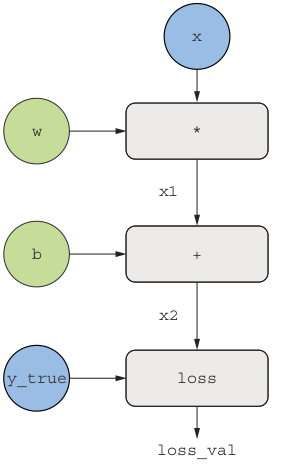
\includegraphics[scale=0.5]{figuras/grafo_computacional.png}
    \caption{Grafo computacional}
\end{figure}
Onde $x$ e $y_{true}$ são as variáveis de entrada, e $w$ $b$ são
os parâmetros da rede neural artificial. 
Sabendo que cada uma das duas rodas sequem as equações:
\begin{align}
    \frac{1}{r}
    \begin{bmatrix}
        \sin(\alpha + \beta) &  -\cos(\alpha + \beta) & -l\cos(\beta) \
    \end{bmatrix}
    \dot{\xi}
    = \phi \\
    \begin{bmatrix}
        \cos(\alpha + \beta) &  \sin(\alpha + \beta) & -l\sin(\beta) \
    \end{bmatrix}
    \dot{\xi}
    = 0 
\end{align}
Através dessa estrutura de dados e das equações, foi
modelado os parâmetros de uma rede neural artificial,
onde $\alpha$,$\beta$,$r$,$l$ são parâmetros da rede neural,
$\dot{\xi}$ a entrada do modelo e $\phi$ e $0$  são a saídas desejadas.
O grafo computacional com essas operações são representadas por essas equações:

\begin{align}
    \gamma = \alpha + \beta \\
    \cos_{\gamma} = \cos(\gamma) \\
    \sin_{\gamma} = \sin(\gamma) \\
    l_{\phi} = \frac{-l\cos(\beta)}{r} \\
    l_{0} = l\sin(\beta) \\
    W_{\phi_1} = \frac{\sin_{\gamma}}{r} \\
    W_{\phi_2} = \frac{-\cos_{\gamma}}{r} \\
    W_{\phi} = \textbf{tensor\_concat\_h}(_{\phi_1},_{\phi_2}, l_{\phi})\\
    W_{0} = \textbf{tensor\_concat\_h}(\cos_{\gamma},\sin_{\gamma},  l_{0}) \\
    W = \textbf{tensor\_concat\_v}( W_{\phi}, W_{0} ) \\
    y_{\textbf{pred}} =  W \times  \dot{\xi} 
\end{align}
onde cada variável é um tensor, e a
função \textbf{tensor\_concat\_h} junta os tensores horizontalmente:
\begin{align}
    \alpha = 
    \begin{bmatrix}
         \alpha_{1,1} \\
         \alpha_{2,1}
    \end{bmatrix}
    \\
    \beta =
    \begin{bmatrix}
        \beta_{1,1} \\
        \beta_{2,1}
   \end{bmatrix}\\
   \textbf{tensor\_concat\_h}( \alpha, \beta ) =
   \begin{bmatrix}
    \alpha_{1,1} && \beta_{1,1} \\
    \alpha_{2,1} &&  \beta_{2,1} \\
\end{bmatrix}
\end{align}
e \textbf{tensor\_concat\_v} junta os tensores verticalmente:
\begin{align}
    \alpha = 
    \begin{bmatrix}
         \alpha_{1,1} \\
         \alpha_{2,1}
    \end{bmatrix}
    \\
    \beta =
    \begin{bmatrix}
        \beta_{1,1} \\
        \beta_{2,1}
   \end{bmatrix}\\
   \textbf{tensor\_concat\_v}( \alpha, \beta ) =
   \begin{bmatrix}
    \alpha_{1,1} \\
    \alpha_{2,1} \\
    \beta_{1,1} \\
    \beta_{2,1} \\
\end{bmatrix}
\end{align}
Perceba que $W_{\phi}$ representa as equações das rodas, onde
o valor desejado são as velocidades angulares $\phi_1,\phi_2$ das rodas:

\begin{align}
    W_{\phi} = 
    \begin{bmatrix}
        \frac{\sin(\alpha_{1,1} + \beta_{1,1})}{r_1} &  \frac{-\cos(\alpha_{1,2} + \beta_{1,2})}{r_1} & \frac{-l\cos(\beta_{1,3})}{r_1} \\
        \frac{\sin(\alpha_{2,1} + \beta_{2,1})}{r_2} &  \frac{-\cos(\alpha_{2,2} + \beta_{2,2})}{r_2} & \frac{-l\cos(\beta_{2,3})}{r_2}
    \end{bmatrix}
\end{align}

Na prática estamos fazendo uma regressão não linear para encontrar
os parâmetros de uma transformação linear, então podemos também pensar em
grafo de computacional mais simples, que encontra  a melhor transformação
linear que satisfaça o conjunto de dados coletados,
Neste caso podemos modelar o grafo de maneira mais simples: $\phi=W \times \dot{\xi}$,
onde cada peso é $W_{i,j}$ é encontrado separadamente. Ambos os modelos foram
treinados e foram discutidos na sessão de experimentos e resultados.


\section{pre-processamento dos dados e treinamento do modelo}

% Cap. 5 - Implementação
% %%
%% Capítulo 4: Figuras, gráficos e tabelas
%%

\mychapter{Implementação}
\label{Cap:Implementacao}
Lorem ipsum dolor sit amet, consectetur adipiscing elit. Morbi tristique, orci mollis tincidunt dignissim, purus lectus molestie odio, vitae pharetra nisi sapien et justo. Fusce consequat et elit condimentum tincidunt. In eu venenatis tortor, quis lobortis tellus. Mauris tincidunt gravida ante. Pellentesque ante elit, lacinia interdum bibendum sed, cursus non orci. Ut et diam nec justo efficitur tincidunt. Fusce convallis facilisis varius. Integer tempor hendrerit maximus.

\begin{algorithm}
%% \SetLine
\Entrada{$x$: vetores de valores; $y$ = $L(x)$; $p$: valor de entrada a ser calculado }
\Saida{$s$ = $L(p)$}
$n \leftarrow \mathtt{comprimento}(x)$\;
$s \leftarrow 0$\;
\Para {$i=1$ \Ate $n$} {
	$L \leftarrow 1$\;
	\Para {$j=1:1:n$} {
		\Se{$i \neq j$} {
			$L \leftarrow L* \left( \dfrac{p-x[j]}{x[i]-x[j]} \right) $
		}
	}
	$s \leftarrow s + L*y[i]$\;
}
\Retorna $s$\;
\caption{Algoritmo para interpolação de Lagrange.}
\label{algo:1}
\end{algorithm}

\begin{algorithm}
%% \SetLine
\Entrada{$a$: valor inicial; $b$: valor final; $n$: número de subintervalos (deve ser múltiplo de 2)  }
\tcc{A função a ser integrada é definida em uma função denominada \texttt{f}, fora do escopo deste algoritmo.}
\Saida{$I$ = integral de \texttt{f} entre $a$ e $b$}
$h \leftarrow$ $\dfrac{b-a}{n}$\;
$x[1] \leftarrow a$\;
$y[1] \leftarrow f(a)$\;
$I \leftarrow 0$\;
$k \leftarrow 2$\;
\Enqto {$k <= n$} {
	$x[i] \leftarrow x[i-1] + h$\;
	$y[i] \leftarrow f(x[i])$\;
	\eSe{$i \% 2 = 0$} {
		$I \leftarrow I + 4*y[i]$\;
	}
	{
		$I \leftarrow I + 2*y[i]$\;
	}
	$k = k+1$\;
}
$x[n+1] \leftarrow b$\;
$y[n+1] \leftarrow f(x[i+1])$\;
$I \leftarrow I + \dfrac{h}{3}*(I + y[n+1])$\;
\Retorna $I$\;
\caption{Algoritmo para a integração pelo primeiro método de Simpson.}
\label{algo:2}
\end{algorithm}



\section{Nulla molestie libero sed}
\label{Sec:expressoesMatematicas}

\begin{eqnarray} \label{eq:PDF:RSR}
  p \left( \gamma \right) & = & \frac{1}{2} \sqrt{\frac{M}{\gamma \bar{\gamma}_{b}}} \frac{1}{ \prod_{i=1}^M {\sqrt{\tilde{\gamma}_i}}}
  \int_0^{\sqrt{M \delta}} \int_0^{\sqrt{M \delta} - r_M } \cdots
  \int_0^{\sqrt{M \delta} - \sum_{i = 3}^M {r_i } } \nonumber \\
  & & p \left( {\frac{\sqrt{M \delta} - \sum_{i = 2}^M {r_i }}{\sqrt{\tilde{\gamma}_1}} ,
  \frac{r_2}{\sqrt{\tilde{\gamma}_2}} , \ldots ,\frac{r_M}{\sqrt{\tilde{\gamma}_M}} } \right)
  \, dr_2 \cdots dr_{M-1} \, dr_M
\end{eqnarray}
% sem linha em branco
ou:
% sem linha em branco
\begin{equation} \label{eq:TrCGI}
  T(r) = \frac{1}{f_m}
  \left( \frac{\pi}{2} \sum_{i=1}^M
  {\tilde{r}_i^2 \dot{\varsigma}_i^2}\right)^{-1/2}
  \frac
  {\begin{array}{ll}
  \int_0^{\rho \sqrt{M}} \int_0^{\rho \sqrt{M} - r_M } \cdots
  \int_0^{\rho \sqrt{M} - \sum_{i = 3}^M {r_i } } \int_0^{\rho \sqrt{M} -
  \sum_{i = 2}^M {r_i } }  \\
  p \left( {\frac{r_1}{\tilde{r}_1} ,
  \frac{r_2}{\tilde{r}_2} , \ldots ,\frac{r_M}{\tilde{r}_M} } \right)
  \, dr_1 \, dr_2 \cdots dr_{M-1} \, dr_M \\ \end{array}}
  {\begin{array}{ll}
  \int_0^{\rho \sqrt{M}} \int_0^{\rho \sqrt{M} - r_M } \cdots
  \int_0^{\rho \sqrt{M} - \sum_{i = 3}^M {r_i } } \\
  p \left( {\frac{\rho \sqrt{M} - \sum_{i = 2}^M {r_i }}{\tilde{r}_1} ,
  \frac{r_2}{\tilde{r}_2} , \ldots ,\frac{r_M}{\tilde{r}_M} } \right)
  \, dr_2 \cdots dr_{M-1} \, dr_M \\ \end{array}}
\end{equation}


\begin{equation}
y = g(x) = g(x_{PO}) + \left.\frac{dg}{dx}\right|_{x=x_{PO}}
\frac{(x-x_{PO})}{1!} + \left.\frac{d^2g}{dx^2}\right|_{x=x_{PO}}
\frac{(x-x_{PO})^2}{2!} + \cdots
\label{Eq:Taylor}
\end{equation}



% Cap. 6 - Experimentos e Resultados
%%
%% Capítulo 4: Figuras, gráficos e tabelas
%%

\mychapter{Experimentos e Resultados}
\label{Cap:ExperimentosResultados}
Neste trabalho foram feitos dois experimentos em relação a criação
de um modelo cinemático para o robô, o primeiro experimento foi o
treinamento de um modelo de rede neural simples, onde o algoritmo
de aprendizado supervisionado deve buscar uma transformação linear,
que mapeia velocidade linear e angular do robô para as velocidades
angulares das rodas sem levar em consideração as equações das rodas,
o segundo experimento é o treinamento de um modelo cujo os parâmetros
são constantes das equações rodas, onde o algoritmo de aprendizado
de máquina deve realizar uma regressão não linear para encontrar
estes parâmetros, por fim é resolvida analaticamente a cinemática
com a finalidade de comparar com os dois modelos. Em relação ao controlador,
foi implementado o controlador Vieira e encontradas as constantes do P.I.D
empiricamente.


\section{Experimentos com a Cinemática}
Em todos os treinamentos dos modelos
de rede neural artificial foi utilizado o algoritmo de otimização
RMSprop com uma taxa de aprendizado de 0,0001, um momentum $m =0$,
foi utilizado o \textit{Framework pytorch}, para a criação dos
grafos computacionais e treinamento dos modelos. \textit{Pytorch}
permite a criação e prototipagem de um modelo de aprendizagem de
máquina na linguagem \textit{Python} ao mesmo tempo que possui
uma versão em C++ e \textit{Rust}, permitindo criar aplicações
bastante performáticas. Em nosso Experimentos a execução do modelo
em \textit{Rust} é em média 2 vezes mais rápido do que a mesma implementação
em \textit{Python}, para se chegar a esse número foi executado 10 mil vezes o cálculo
da cinemática, em um \textit{notebook} com processador de 4 núcleos \textit{AMD Ryzen 5 2500U},
sem placa de vídeo dedicada. Para a criação dos modelos foi executado o
algoritmo de coleta de dados obtendo conjunto com 10 mil
pontos. Durante o treinamento é dividido este conjunto de dados
onde 60\% dos dados são utilizados para treinamento e 40\% foi utilizado
apenas para avaliação, ou seja, a rede não possui informação sobre esses
pontos durante o treinamento, nas figuras \ref{fig:error:quadratico:nao:linear} e
\ref{fig:error:quadratico:linear} a linha vermelha representa o erro de
Avaliação, e a linha azul representa o erro durante o treinamento,
a métrica de erro utilizada para o treinamento e avaliação
foi o erro quadrático médio.

\begin{figure}[H]
    \label{fig:error:quadratico:nao:linear}
    \centering
    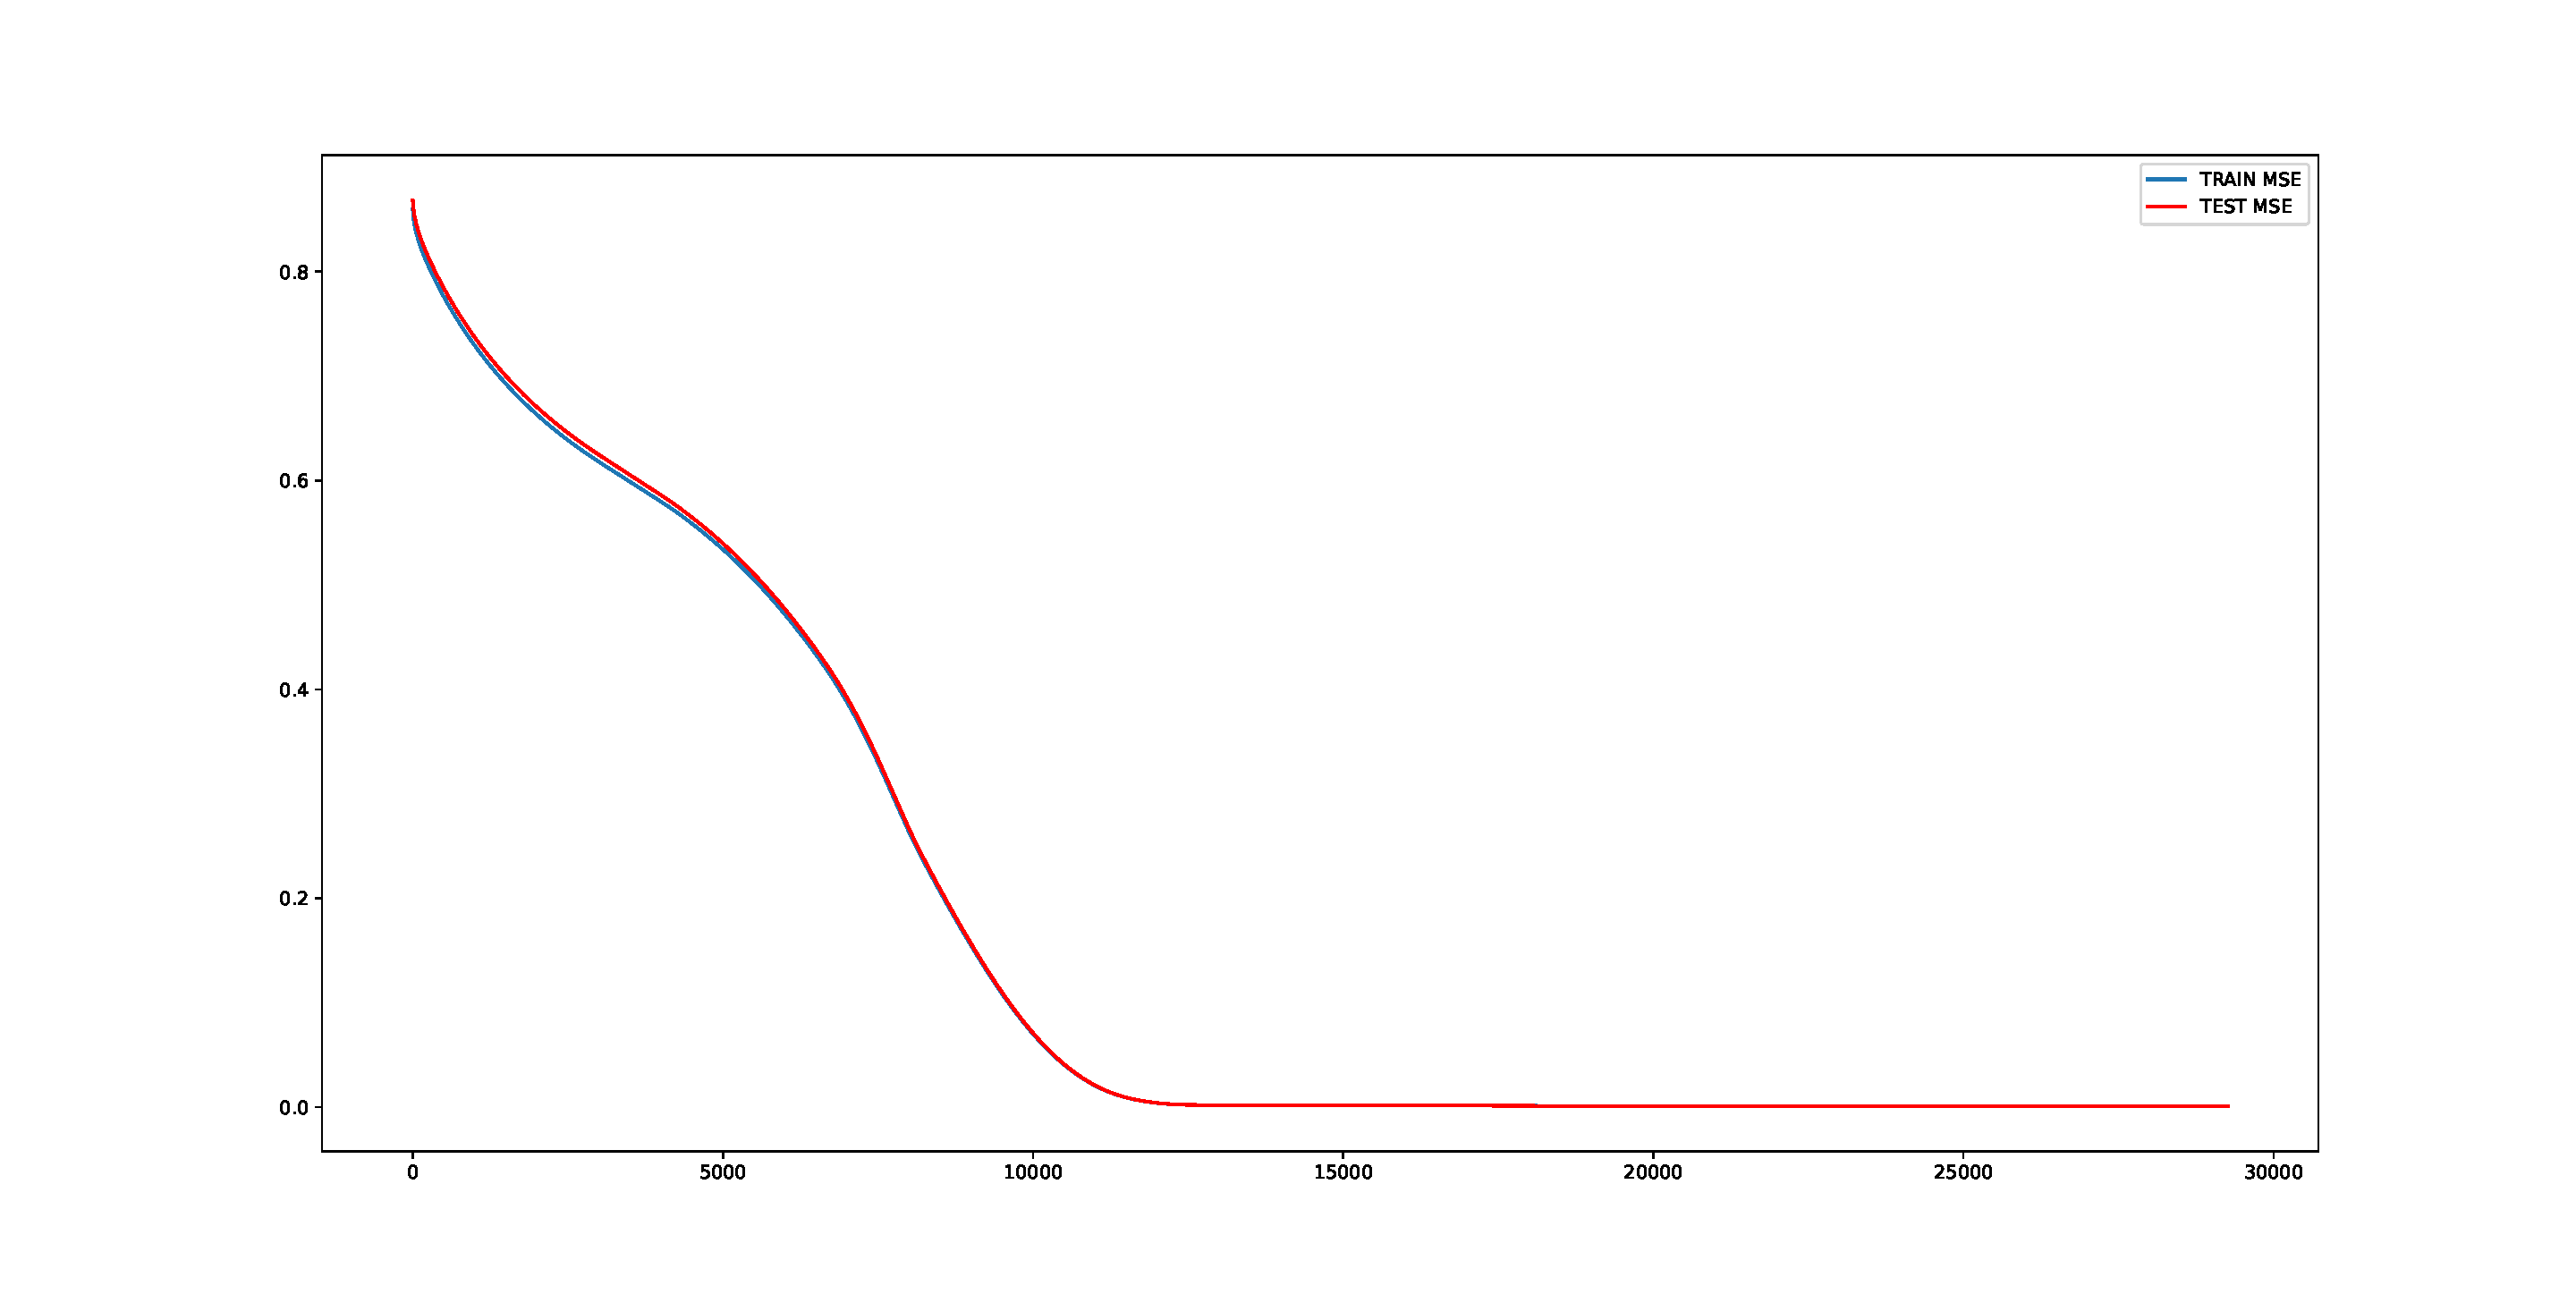
\includegraphics[scale=0.3]{figuras/MSE_error_non_linear.pdf}
    \caption{Erro Médio quadrático regressão não linear}
\end{figure}

\begin{figure}[H]
    \label{fig:error:quadratico:linear}
    \centering
    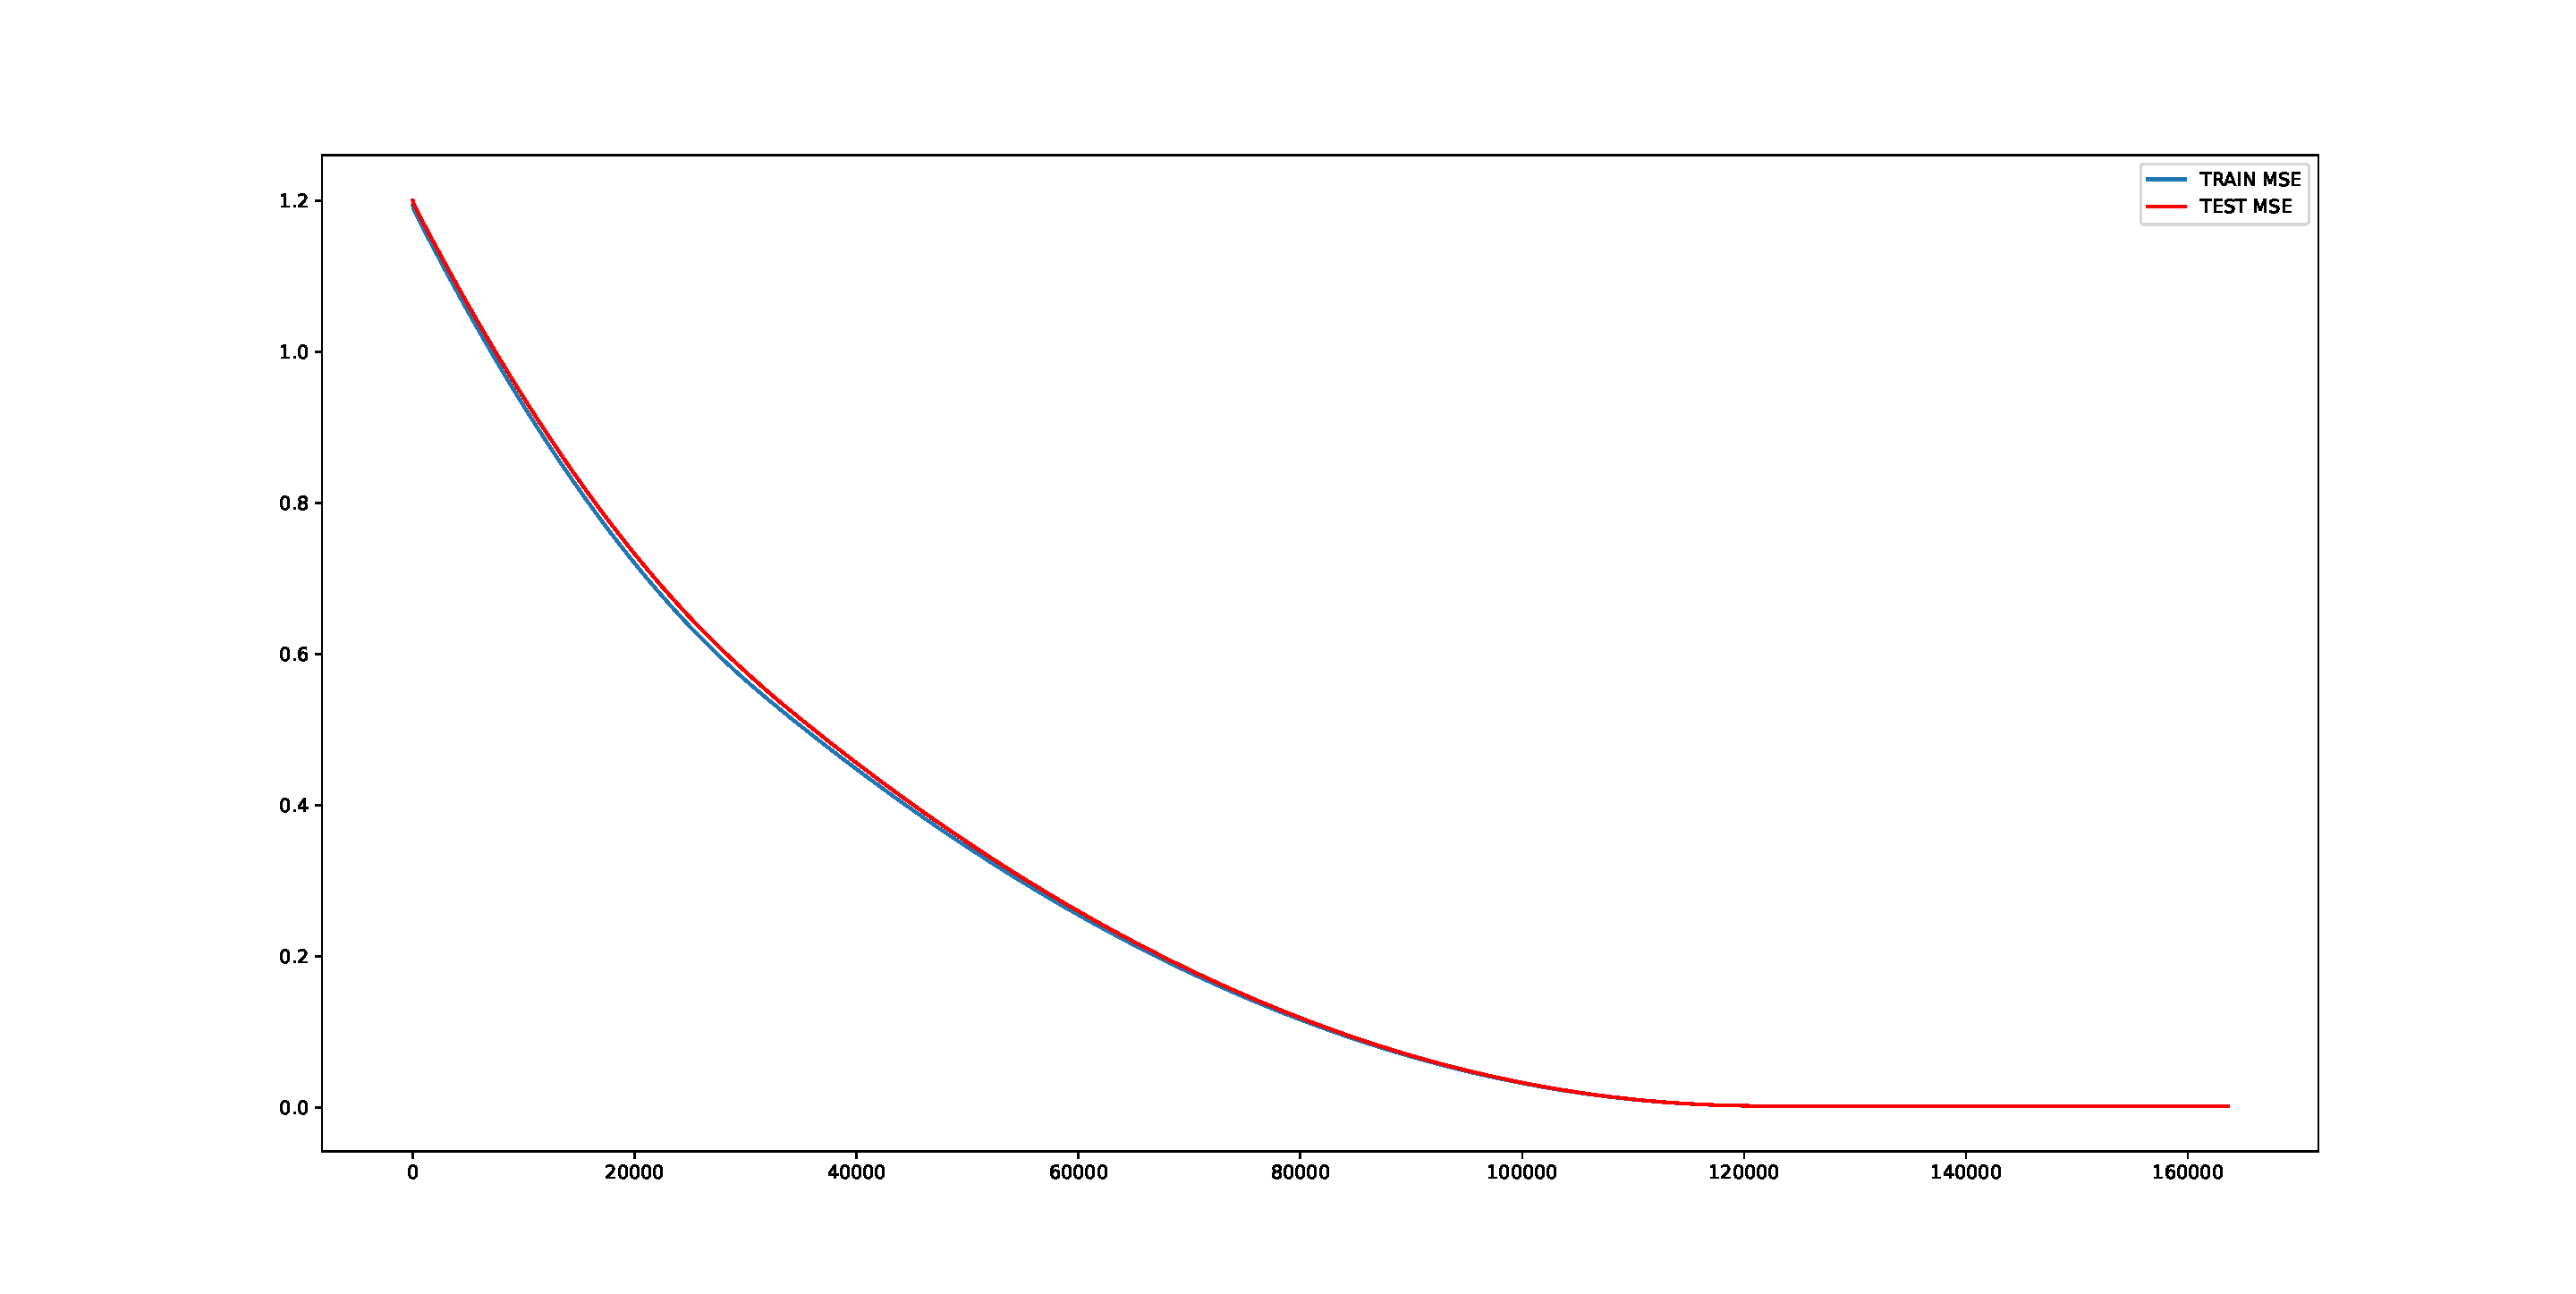
\includegraphics[scale=0.3]{figuras/mse_error_linear.pdf}
    \caption{Erro Médio quadrático regressão linear}
\end{figure}

Para teste dos modelos cinemáticos foram coletados mais 10 mil pontos,
mas dessa vez com o robô podendo variar a velocidade angular das rodas
para até 5 vezes o raio da roda, ou seja $V_{MAX}=5$, no entanto ao invés
de coletar dados de posição, foi extraído do simulador diretamente a
velocidade do robô.

\begin{figure}[H]
    \label{fig:conj:dados}
    \centering
    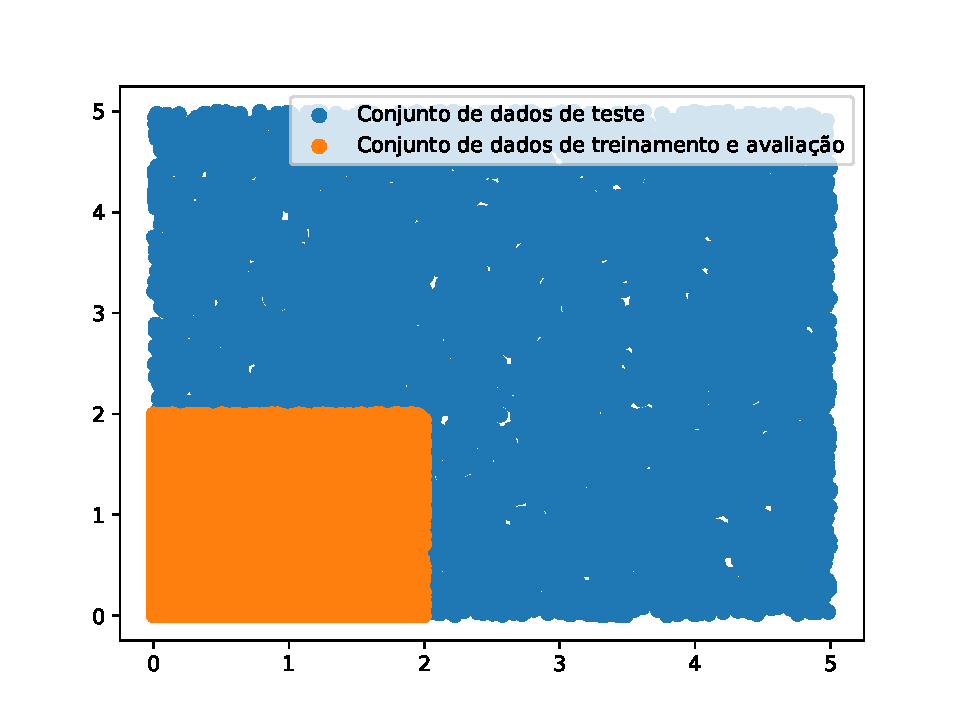
\includegraphics[scale=0.5]{figuras/conj_dados.pdf}
    \caption{Comparação entre os conjuntos de dados}
\end{figure}

Podemos observar que na figura \ref{fig:conj:dados} que o conjunto
de dados para treinamento e avaliação do modelo 
é um sub conjunto do conjunto de testes. Foi calculado o erro quadrático
médio dos modelos em relação ao conjunto de testes gerando a
tabela \ref{table:mse:test}


\begin{table}[H]
    \label{table:mse:test}
    \centering
    \begin{tabular}{c|c}
        \hline
        Erro quadrático médio & modelo \\
        \hline
        0,0037 & modelo regressão linear \\
        \hline
        0,0032 & modelo regressão não linear \\
        \hline
        0,0027 & modelo analítico \\
        \hline
    \end{tabular}
    \caption{teste dos modelos}
\end{table}

Como se sabe o significado físico dos parâmetros do modelos gerados
através de algoritmos de aprendizado de máquina, então na figura
\ref{fig:parametros:da:cinemantica} mostra os valores encontrados
sendo $W_{A}$ os valores do calculo analítico, $W_{K}$ e $W_{L}$ 
são os valores obtidos através da regressão não linear e linear
respectivamente. A tabela \ref{table:param:kinematic} mostra os valores
dos parâmetros das rodas após a regressão não linear, e a tabela
\ref{table:param:analytic} mostra os valores dos parâmetros da
solução analítica, em ambas as tabelas os ângulos estão medidos
em graus, e os raio da roda $r$ e distância $l$ estão em metros.
 
\begin{figure}[H]
    \label{fig:parametros:da:cinemantica}
    \begin{align*}
        W_{A} = 
        \begin{bmatrix}
            12,1212 &  0,0000 & 3,5307 \\
            12,1212 &  0,0000 & -3,5307 \\
        \end{bmatrix}\\
        W_{K} = 
        \begin{bmatrix}
            12,2294 &  -0,0291 & 3,7330 \\
            12,1241 &  -0,1347 & -3,5121
        \end{bmatrix}\\
        W_{L} = 
        \begin{bmatrix}
            12.2262 &  -1.3070 & 3.5472 \\
            12.1198 &  -4.4313 & -4.1472
        \end{bmatrix}\\
    \end{align*}
    \caption{Modelos cinemáticos}
\end{figure}

\begin{table}[H]
    \label{table:param:kinematic}
    \centering
    \begin{tabular}{c|c|c|c|c}
        \hline
         $\alpha$ &$\beta$ &$l$ &$r$ & roda \\
        \hline
        115,6515 &-25,8002 &-0,3389 &0,0818 & roda esquerda \\
        \hline
        62,3091  &27,1352 &0,3254 &0,0825 & roda direita \\
        \hline
    \end{tabular}
    \caption{parâmetros das rodas após a regressão não linear}
\end{table}
Perceba que o angulo $\gamma = \alpha + \beta$ do modelo gerado pela regressão não
linear foi de $\gamma_{k_1} = 115,6515 -25,8002  = 89,8513$ e 
$\gamma_{k_2} = 62,3091 +27,1352 = 89,4443$
\begin{table}[H]
    \label{table:param:analytic}
    \centering
    \begin{tabular}{c|c|c|c|c}
        \hline
         $\alpha$ &$\beta$ &$l$ &$r$ & roda \\
        \hline
        90 & 0 &-0,2912 &0,0825 & roda esquerda \\
        \hline
        -90  & 180 & 0,2912 &0,0825 & roda direita \\
        \hline
    \end{tabular}
    \caption{parâmetros das rodas modelo analítico}
\end{table}


Como dito anteriormente foi utilizado o controlador Vieira,
cujo os parâmetros dos P.I.Ds foram adquiridos empiricamente,
visando minimizar o sobre-sinal do controlador de velocidade linear,
os valores podem ser vistos na tabela \ref{table:pid:}.

\begin{table}[H]
    \label{table:pid:}
    \centering
    \begin{tabular}{c|c|c|c}
        \hline
        P & I & D & tipo de controlador \\
        \hline
        0,05145 & 0,01769 & 0,60529 & velocidade linear \\
        \hline
        0,4 & 0,015 & 0 & velocidade angular \\
        \hline
    \end{tabular}
    \caption{parâmetros P.I.D}
\end{table}

Para avaliar o sistema de controle, com os diferentes modelos
cinemáticos, foi posicionado um alvo e observado o robô no seu
trabalho em chegar até alvo mensurando a distância e o angulo do robô até
o alvo, essas duas medidas foram escolhidas pois 
estes são os valores a serem minimizados pelo controlador Vieira,
o alvo foi posicionado em quatro lugares diferentes como mostra a figura
\ref{fig:robo:e:4:alvos}.

\begin{figure}[H]
    \label{fig:robo:e:4:alvos}
    \centering
    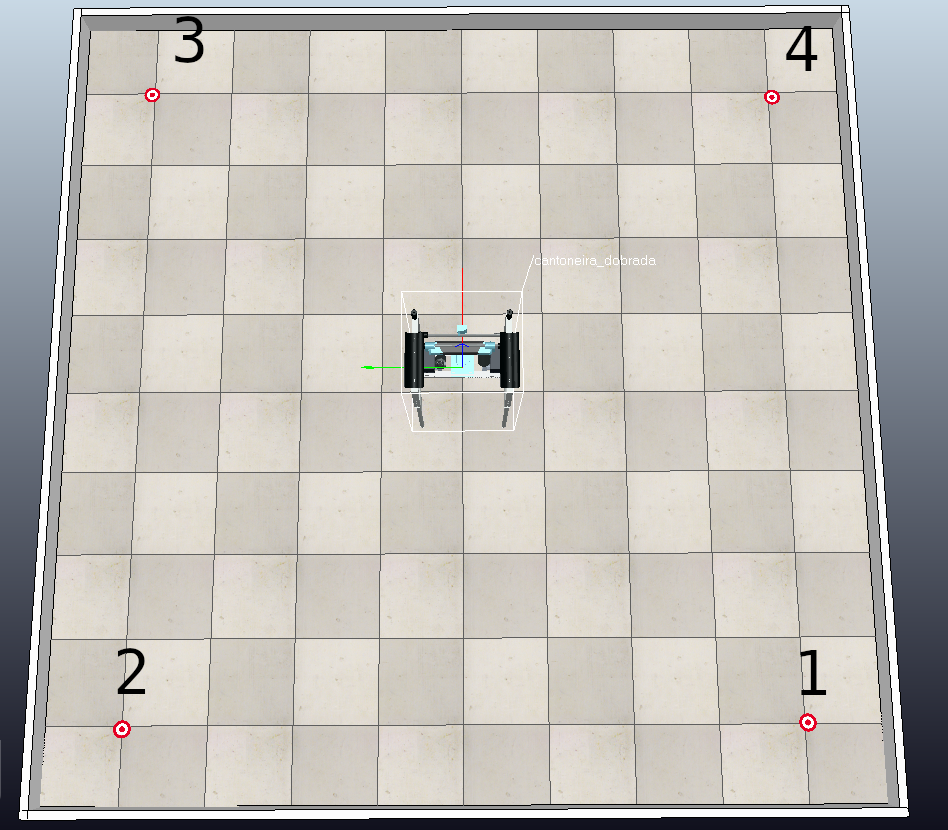
\includegraphics[scale=0.3]{figuras/robo_e_alvo.png}
    \caption{Robô e alvo}
\end{figure}

\begin{figure}[H]
    \centering
    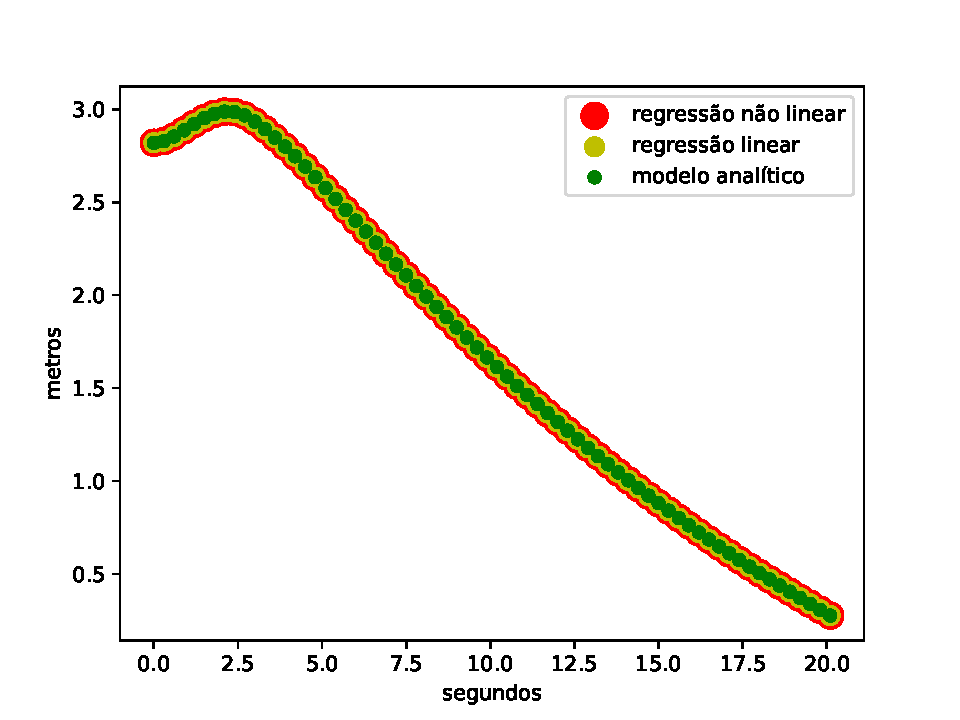
\includegraphics[scale=0.45]{figuras/distance_over_time_1.pdf}
    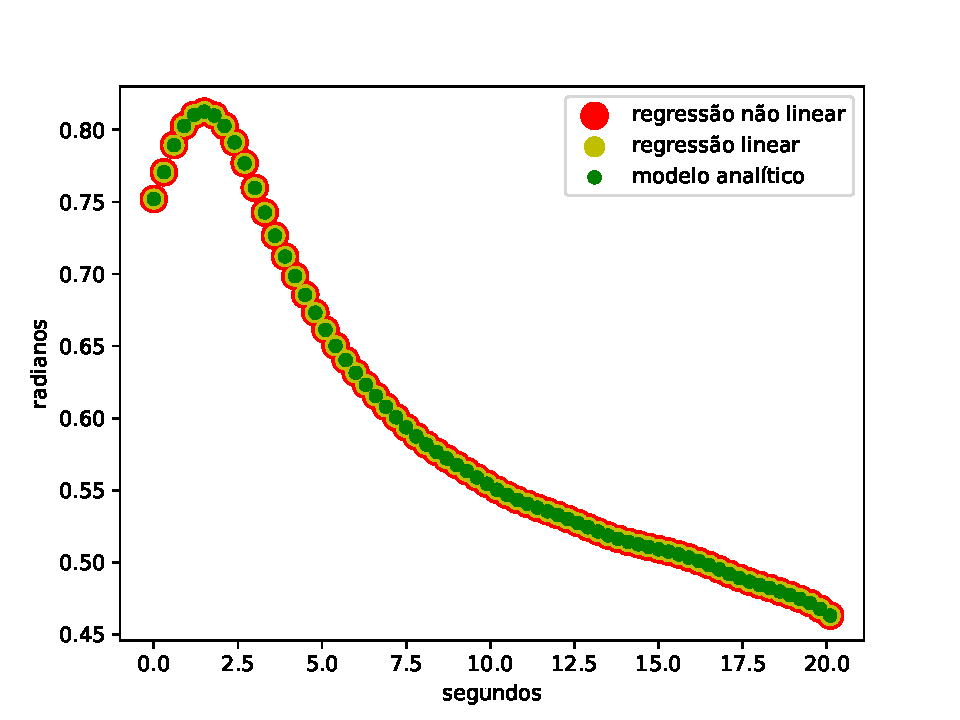
\includegraphics[scale=0.45]{figuras/angle_over_time_1.pdf}
    \caption{Angulo e distância observada no alvo 1}
\end{figure}

\begin{figure}[H]
    \centering
    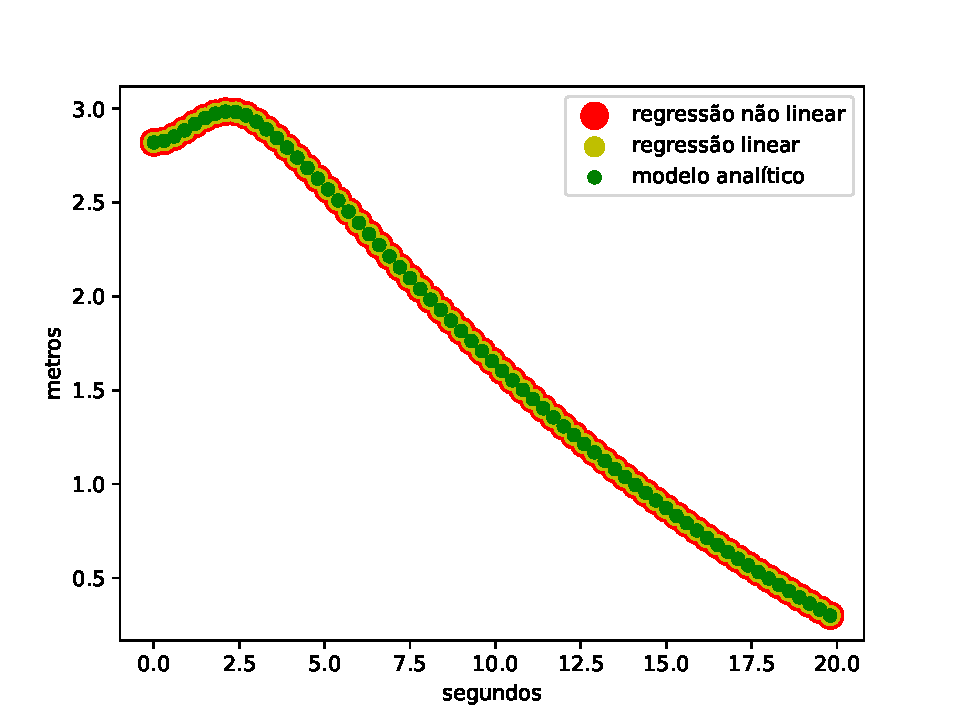
\includegraphics[scale=0.45]{figuras/distance_over_time_2.pdf}
    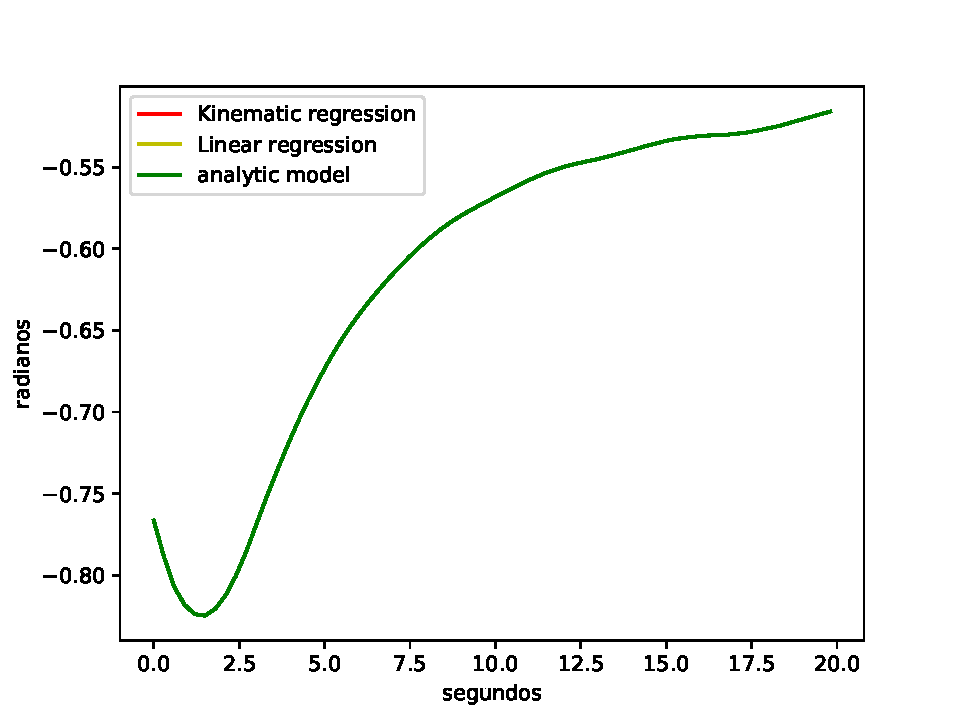
\includegraphics[scale=0.45]{figuras/angle_over_time_2.pdf}
    \caption{Angulo e distância observada no alvo 2}
\end{figure}

\begin{figure}[H]
    \centering
    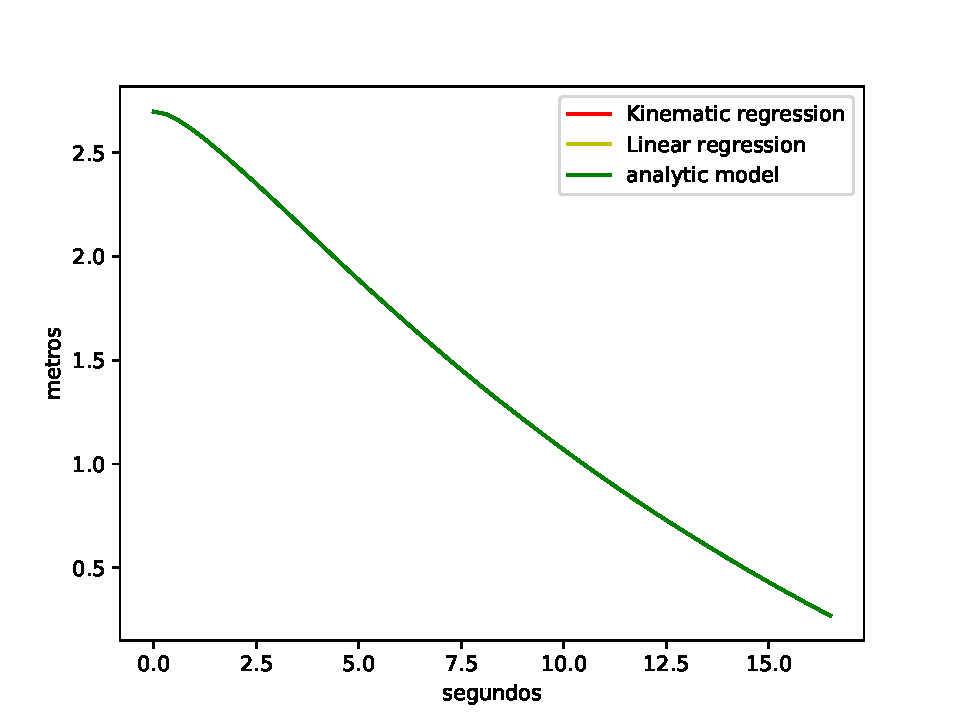
\includegraphics[scale=0.45]{figuras/distance_over_time_3.pdf}
    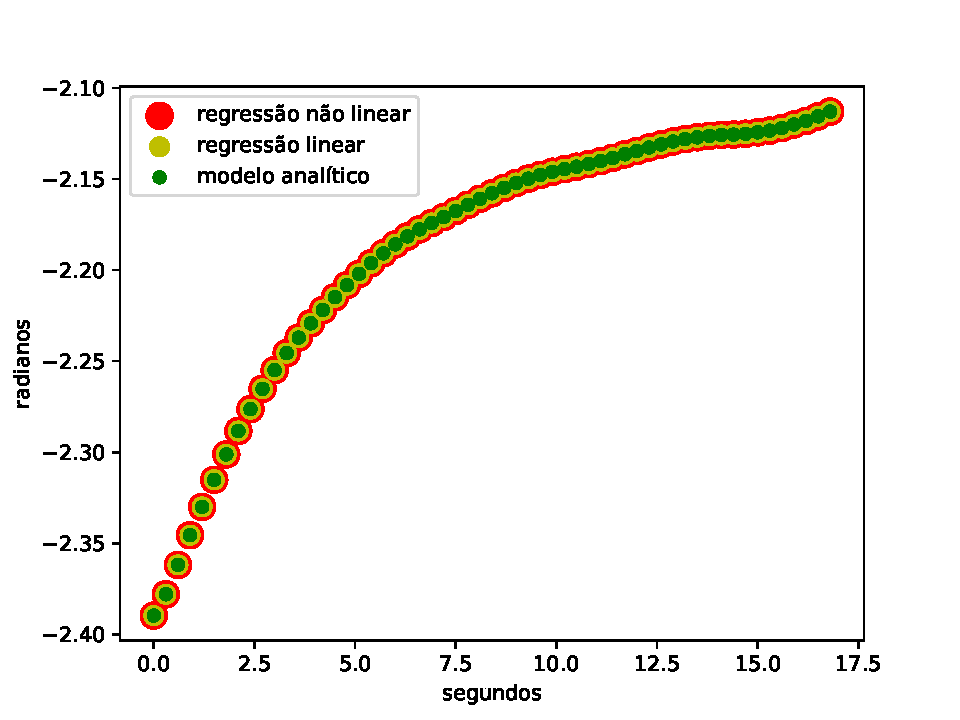
\includegraphics[scale=0.45]{figuras/angle_over_time_3.pdf}
    \caption{Angulo e distância observada no alvo 3}
\end{figure}

\begin{figure}[H]
    \centering
    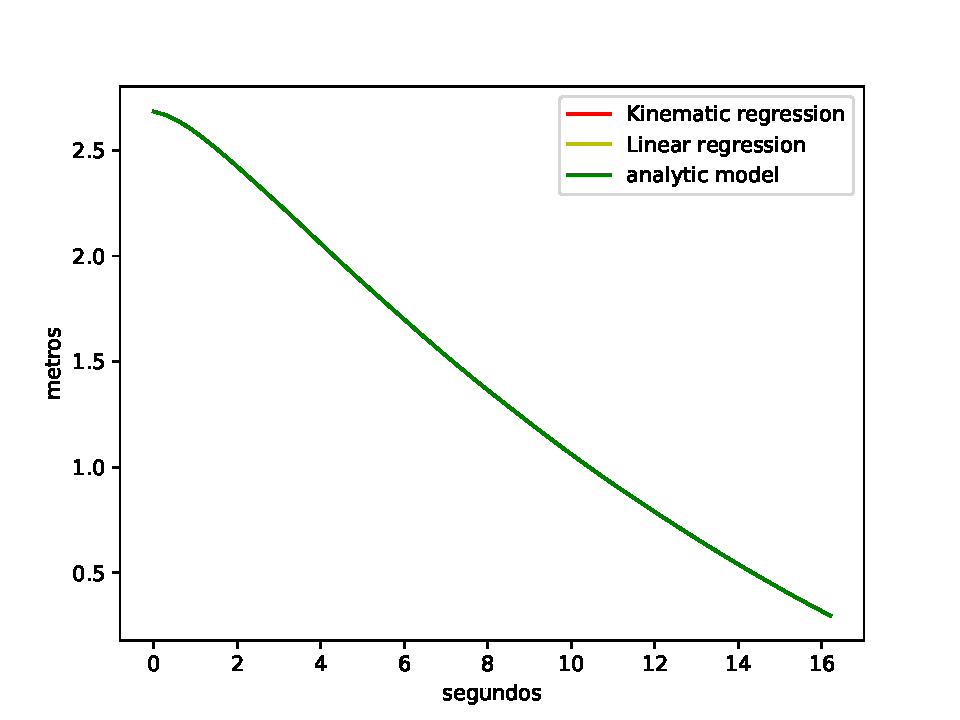
\includegraphics[scale=0.45]{figuras/distance_over_time_4.pdf}
    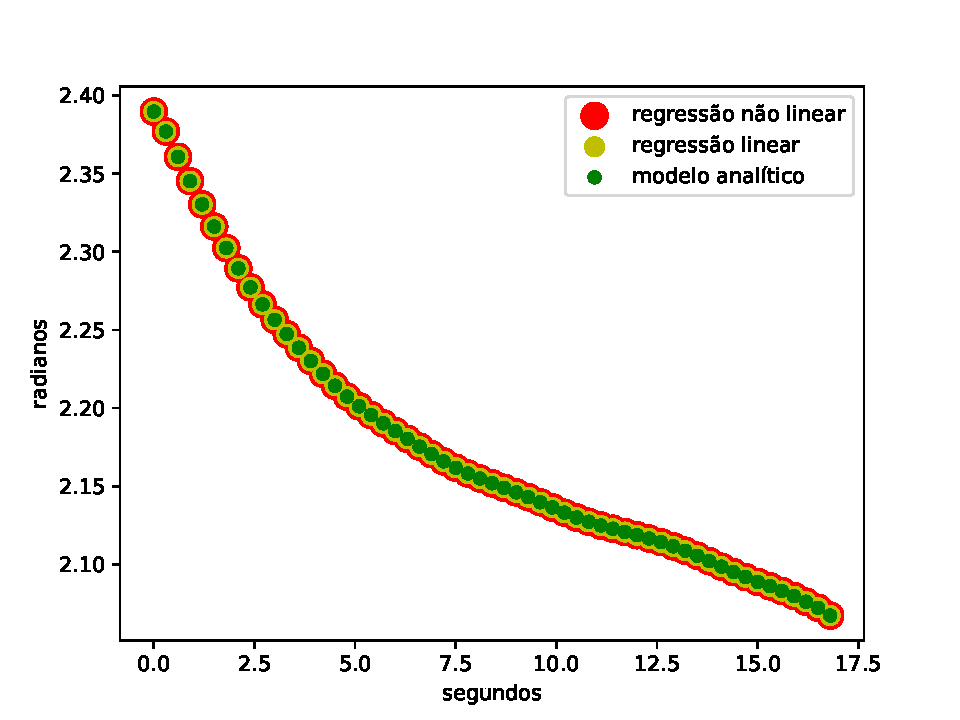
\includegraphics[scale=0.45]{figuras/angle_over_time_4.pdf}
    \caption{Angulo e distância observada no alvo 4}
\end{figure}

Perceba os pontos dos modelos obtidos através da regressão e o modelo analítico
estão sobrepostos.

\section{Discussão dos Experimentos}
Na observação do robô em seu trabalho de chegar até o alvo, os modelos
obtidos através da regressão linear e não linear tiveram respostas
idênticas ao modelo analítico, também na tabela do erro quadrático médio \ref{table:mse:test},
os valores ficaram nas mesmas casas decimais, através desses dois fatos
podemos dizer que os modelos são equivalentes, outro ponto interessante é
observar a generalização do modelos, uma vez que o conjunto do treinamento
é um sub conjunto do conjunto de testes o que nos dá segurança em aplicar
o modelo em dados nunca vistos, em aprendizado de máquina supervisionada
muitas vezes é feita uma escolha em generalização e otimização, onde um
modelo mais otimizado ao conjunto de dados de treinamento tende a não ir
bem e dados fora desse conjunto, no entanto ao modelarmos o sistema cinemático
do robô ao mesmo tempo que modelamos os pesos de uma rede neural artificial,
mostramos que otimizar os parâmetros de uma rede neural modelada estamos
também aumentando a sua generalização.
Comparando os modelos de aprendizado, podemos observar que a regressão
linear durou cento e sessenta mil iterações, já a regressão não linear parou de reduzir
o erro com trinta mil iterações, apesar do tempo de treinamento está
fortemente relacionado om os valores iniciais da rede, a regressão não
linear teve mais duas equações iguais a zero que ajudou a guiar o erro
mais rápido. Outro ponto interessante de se notar na figura \ref{fig:parametros:da:cinemantica}
é que os pesos da regressão linear afirmam existir uma contribuição negativa
de velocidade linear no eixo y do robô, algo também observado no modelado de
regressão não linear, só que com valores inferiores devido as equações,
talvez estes valores deve-se a aproximação da velocidade por meio da variação
de posição sobre variação do tempo ou algum fator dinâmico da simulação.
Comparando os valores das tabelas \ref{table:param:kinematic} e \ref{table:param:analytic}
podemos perceber que a rede convergiu o angulo $\gamma = \alpha + \beta$,
uma vez que o gamma analítico é  $\gamma_{A} = 90$ e o gamma do modelo
de regressão não linear foi de $\gamma_{K} = 89$. O modelo de aprendizado
de máquina é resultado dos seus dados, como existe uma pequena velocidade
no eixo y do robô, a rede reajustou os parâmetros $l$ e $\beta$ de modo que
representa-se os dados, apensar do modelo não ter encontrado os ângulos,
$\beta, \alpha$ próximos da solução analítica, os raios da rodas estão
com valores muito próximos e a distância $l$ está a uma diferença de
centímetros da solução analítica. Este trabalho também buscar uma solução
que pode-se sem implementada em um computador com limitação de
processamento e memória, então se consideramos que o treinamento poder ser
realizado em outro computador, onde o robô enviaria os dados,
por tanto se consideramos só o sistema de controle, o computador apenas
executará o algoritmo do  P.I.D mais a multiplicação de uma matriz da
cinemática que contem 6 elementos, então o computador utilizado não irá precisar de muita memória e processamento,
sendo a parte mais crítica o armazenamento de um buffer durante o algoritmo
da coleta de dados, outro pronto crítico seria o tempo de bateria durante
a coleta de dados, mas considerando que um ciclo de controle esta por volta
de 30 ms, portanto para coletar 10 mil amostras equivale a 300 segundos, ou
seja, 5 minutos.

% Cap. 7 - Conclusão
%%
%% Capítulo 5: Conclusões
%%

\mychapter{Conclusão}
\label{Cap:Conclusao}

Este trabalho visou aplicar e avaliar sistemas de aprendizado de máquina
na construção de um controlador para um robô móvel de acionamento diferencial
que ajuda pessoas com mobilidade reduzida. Inicialmente foi feito uma
revisão bibliográfica onde concluímos que sistemas de aprendizado de
máquina que substitui um controlador clássico não é uma boa abordagem,
considerando um cenário simples como foi apresentado neste trabalho,
portanto foi utilizado o controlador Frederico. 
Podemos concluir que uma vez treinado a abordagem utiliza pouca memória,
sendo a coleta de dados o momento mais crítico. Por fim podemos concluir
que resolver o problema da forma clássica, ou seja resolvendo a cinemática
do modelo e criando um controlador clássico é a forma mais simples
de resolver o problema, no entanto com apenas com o conhecimento das equações,
podemos modelar um grafo computacional que encontre os parâmetros das
equações de modo que a solução equivale ao modelo analítico, um fato
interessante que precisa ser melhor investigado.

% Referências bibliogáficas (geradas automaticamente)
% Aqui, o comando \phantomsection é utilizado para auxiliar o pacote "hyperref" a fazer a
% referência correta dos links das referências bibliográficas com a página respectiva.
% Caso seja tirado, o "hyperref" irá apontar o link das referências bibliográficas para a
% última subseção da conclusão.
\phantomsection
\addcontentsline{toc}{chapter}{Referências bibliográficas}
\bibliography{bibliografia/bibliografia}

\appendix

%Apêndice A
%%
%% Capítulo 5: Conclusões
%%

\mychapter{Informações adicionais}
\label{Cap:apendice}

Lorem ipsum dolor sit amet, consectetur adipiscing elit. Morbi tristique, orci mollis tincidunt dignissim, purus lectus molestie odio, vitae pharetra nisi sapien et justo. Fusce consequat et elit condimentum tincidunt. In eu venenatis tortor, quis lobortis tellus. Mauris tincidunt gravida ante. Pellentesque ante elit, lacinia interdum bibendum sed, cursus non orci. Ut et diam nec justo efficitur tincidunt. Fusce convallis facilisis varius. Integer tempor hendrerit maximus.

Donec pulvinar, libero semper pretium fringilla, arcu ligula iaculis urna, id faucibus ante massa a augue. Ut iaculis fermentum convallis. Vestibulum ac porttitor urna, sit amet dignissim dui. Curabitur sollicitudin tincidunt risus quis vulputate. In in leo ut mi mattis tempor sed non nunc. Sed et velit nibh. Duis mollis lectus risus, ut vestibulum purus semper eu. Donec rhoncus ex sed scelerisque dictum. Praesent sit amet neque accumsan, euismod sapien eget, tincidunt magna. Etiam nec diam ac elit feugiat aliquet. Pellentesque et neque metus. Nulla molestie libero sed ullamcorper mollis. In a risus quis felis eleifend dapibus at mollis odio. Curabitur nisl nibh, placerat ac quam nec, vulputate blandit mauris.

Vestibulum neque lacus, fringilla a urna quis, egestas tincidunt orci. Phasellus rutrum elit at mauris feugiat, non egestas tortor dictum. Aliquam faucibus, velit eu aliquam fermentum, lacus sem pellentesque nibh, et tristique urna nibh eget purus. Morbi vitae felis posuere, rutrum turpis quis, rutrum lorem. Nam lacinia cursus neque sit amet fermentum. Mauris eu mauris diam. Quisque lacinia consequat quam, at convallis urna dignissim eget. Proin sit amet varius sem, vel facilisis purus. Sed non blandit sapien. Sed auctor venenatis nibh eu ornare. Quisque euismod urna ligula, quis vestibulum sapien lacinia vehicula. Aenean sit amet vehicula felis, a imperdiet tellus. Fusce eu sem urna. Integer placerat nibh in purus consectetur mattis. Aliquam erat neque, tincidunt ac porta sit amet, egestas non lacus.


\end{document}
